    % Document Class
    \documentclass[10pt,a4paper]{article}

    % Packages essentiels
    \usepackage[utf8]{inputenc}
    \usepackage[T1]{fontenc}
    \usepackage[french]{babel}
    \usepackage{lmodern}

    % Packages mathématiques
    \usepackage{amsmath}
    \usepackage{amssymb}
    \usepackage{amsthm}
    \usepackage{mathtools}

    % Packages pour les graphiques et figures
    \usepackage{graphicx}
    \usepackage{pgfplots}
    \pgfplotsset{compat=1.18}
    \usepackage{float}
    \usepackage{subcaption}

    % Mise en page et design
    \usepackage[hmargin=2.5cm,vmargin=2cm]{geometry}
    \usepackage{fancyhdr}
    \usepackage{enumitem}
    \usepackage{xcolor}
    \usepackage{titlesec}
    \usepackage{siunitx}
    \usepackage{longtable}
    \usepackage{booktabs}
    \usepackage[colorlinks=true,linkcolor=blue,urlcolor=blue,citecolor=blue]{hyperref}

    % Configuration des en-têtes et pieds de page
    \pagestyle{fancy}
    \fancyhf{}
    \fancyhead[L]{\slshape\nouppercase{\leftmark}}
    \fancyhead[R]{\thepage}
    \renewcommand{\headrulewidth}{0.4pt}

    % Définition des environnements mathématiques
    \newtheorem{theorem}{Théorème}[section]
    \newtheorem{proposition}[theorem]{Proposition}
    \newtheorem{lemma}[theorem]{Lemme}
    \newtheorem{corollary}[theorem]{Corollaire}
    \theoremstyle{definition}
    \newtheorem{definition}[theorem]{Définition}
    \newtheorem{example}[theorem]{Exemple}
    \theoremstyle{remark}
    \newtheorem{remark}[theorem]{Remarque}

    % Configuration des titres de sections
    \titleformat{\section}
    {\normalfont\Large\bfseries}{\thesection}{1em}{}
    \titlespacing*{\section}{0pt}{3.5ex plus 1ex minus .2ex}{2.3ex plus .2ex}

    % Informations du document
    \title{\huge\textbf{Heavy tail, Jumps & Endogeneity in HFT}}
    \author{LAFERTE Edouard \and AIAD Janis}
    \date{Juin 2024}

    \begin{document}
    \begin{titlepage}
        \begin{center}
            \vspace*{2cm}
            
            \includegraphics[width=0.4\textwidth]{École_polytechnique_signature.png}
            

            
            {\huge\bfseries Heavy tail, Jumps and \\[0.4cm] 
            Endogeneity in HFT \par}
            
            \vspace{2cm}
            
            {\Large\textsc{Mémoire de Recherche}\par}
            \vspace{1cm}
            
            {\large
            \begin{tabular}{c}
                \textbf{ROUSSELLE Felix-William}\\[0.2cm]
                \textbf{DEBA Ayouba}\\[0.2cm]
                \textbf{AIAD Janis}
            \end{tabular}\par}
            
            \vspace{1.5cm}
            
            {\large Sous la direction de\par}
            \vspace{0.4cm}
            {\large\textbf{Mathieu ROSENBAUM}\par}
            
            \vfill
            
            {\large Département de Mathématiques Appliquées\\
            École Polytechnique\\[0.4cm]
            Mars 2025\par}
        \end{center}
    \end{titlepage}

    % Page blanche après la page de titre
    \newpage
    \null
    \thispagestyle{empty}
    \newpage

    \begin{abstract}
    \thispagestyle{empty}
    \vspace*{1cm}
    \begin{center}

    \end{center}
    \vspace{1cm}

    Ce court projet vise à initier un pré-traitement statistique d'un dataset tick-by-tick de LOB du Nasdaqavec une vingtaine d'actifs sur plusieurs mois. En particulier, on s'intéresse à la vérification des caractéristiques principales du marché sur les queues lourdes, les jumps et changements de régimes endogènes/éxogènes, ainsi que 
    sur la mémoire longue des ordres de marchés.
    On présente ainsi surtout les résultats et graphes principaux obtenus sur quelques actifs pour donner une idée de la qualité des données.
    Toutes les expériences ont été réalisées sur \url{https://github.com/janisaiad/HFT} pour une reproductibilité, avec une exhaustivité des graphes et résultats pour tout le dataset.
    Le but principal étant de construire un projet long-terme sur 1 an avec ce dataset, cette présentation est davantage à voir comme un état d'avancement du prétraitement du dataset.

    A titre indicatif, la suite du projet personnel consisteraient à unifier l'état de l'art des modèles rough comme conséquences de modèles HFT Hawkes (Quadratic Hawkes vers super-Heston rough).

    \vspace{1cm}
    \textbf{Mots-clés :} Limit Order Book, Trading Haute Fréquence, Modèle Queue Reactive, Impact des News, Microstructure de Marché

\end{abstract}
    \newpage
    \tableofcontents
    \thispagestyle{empty}

    \newpage
    \setcounter{page}{1}
    
    
\section{Données utilisées}
Dans la suite de notre étude, nous étudierons les différents actifs du Nasdaq. Ces actifs correspondent à des entreprises de différents secteurs, allant des géants de la technologie aux entreprises de l'agroalimentaire.

\begin{table}[h!]
\centering
\begin{tabular}{|c|c|c|c|}
\hline
\textbf{Actif} & \textbf{Taille Dataset} & \textbf{Nb Jours} & \textbf{Actions/Jour}\\ \hline
GOOGL & 5.6G & 66 & 2.68e6 \\ \hline
AAPL & 3.1G & 55 & 1.78e6 \\ \hline
AMZN & 3.1G & 55 & 1.78e6 \\ \hline
AAL & 2.2G & 371 & 1.87e5 \\ \hline
MSFT & 2.1G & 55 & 1.21e6 \\ \hline
GT & 2.1G & 371 & 1.79e5 \\ \hline
INTC & 1.5G & 75 & 6.33e5 \\ \hline
IOVA & 1.5G & 371 & 1.28e5 \\ \hline
PTEN & 1.5G & 371 & 1.28e5 \\ \hline
MLCO & 1.4G & 371 & 1.19e5 \\ \hline
PTON & 1.4G & 371 & 1.19e5 \\ \hline
VLY & 1.1G & 371 & 9.37e4 \\ \hline
VOD & 951M & 371 & 8.10e4 \\ \hline
CSX & 619M & 75 & 2.61e5 \\ \hline
WB & 591M & 371 & 5.03e4 \\ \hline
BGC & 591M & 371 & 5.03e4 \\ \hline
GRAB & 454M & 371 & 3.87e4 \\ \hline
KHC & 428M & 66 & 2.05e5 \\ \hline
HLMN & 390M & 371 & 3.32e4 \\ \hline
IEP & 342M & 371 & 2.91e4 \\ \hline
GBDC & 338M & 371 & 2.88e4 \\ \hline
WBD & 327M & 75 & 1.38e5 \\ \hline
PSNY & 312M & 371 & 2.66e4 \\ \hline
NTAP & 228M & 55 & 1.31e5 \\ \hline
GEO & 199M & 89 & 7.07e4 \\ \hline
LCID & 163M & 66 & 7.81e4 \\ \hline
GCMG & 160M & 371 & 1.36e4 \\ \hline
CXW & 108M & 89 & 3.83e4 \\ \hline
\end{tabular}
\caption{Tableau des données du Nasdaq}
\label{tab:donnees_nasdaq}
\end{table}

Les données sont issues de la base de données Databento et ne concernent que la bourse du Nasdaq. On observe une grande disparité dans les volumes de données entre les différents actifs, avec notamment les géants technologiques (GOOGL, AAPL, AMZN) qui génèrent des volumes de données significativement plus importants. Les estimations seront donc naturellement plus précises pour ces actifs plus liquides.
\\
\\
Les données sont sous format de dataframe par journée comprenant toutes les modifications apportées au MBO des trois actifs étudiés. Ce MBO comprend alors:
\begin{itemize}
    \item ts\_recv: timestamp du serveur 
    \item ts\_event: timestamp de l'événement     
    \item instrument\_id: id de l'actif sur les marchés
    \item action: Add(A), Cancel(C), Trade(T)
    \item side: Ask(A), Bid(B)
    \item depth: limite considéree
    \item price: prix
    \item size: taille de l'action réalisée
    \item ts\_in\_delta: temps entre le serveur et l'action
    \item sequence: id de l'action propre à l'actif sur les marchés
    \item bid{a}\_px\_0x: prix à la limite x côté bid
    \item bid\_sz\_0x: taille de la file d'attente à la limite x côté bid
\end{itemize}

\begin{figure}[h!]
\centering
    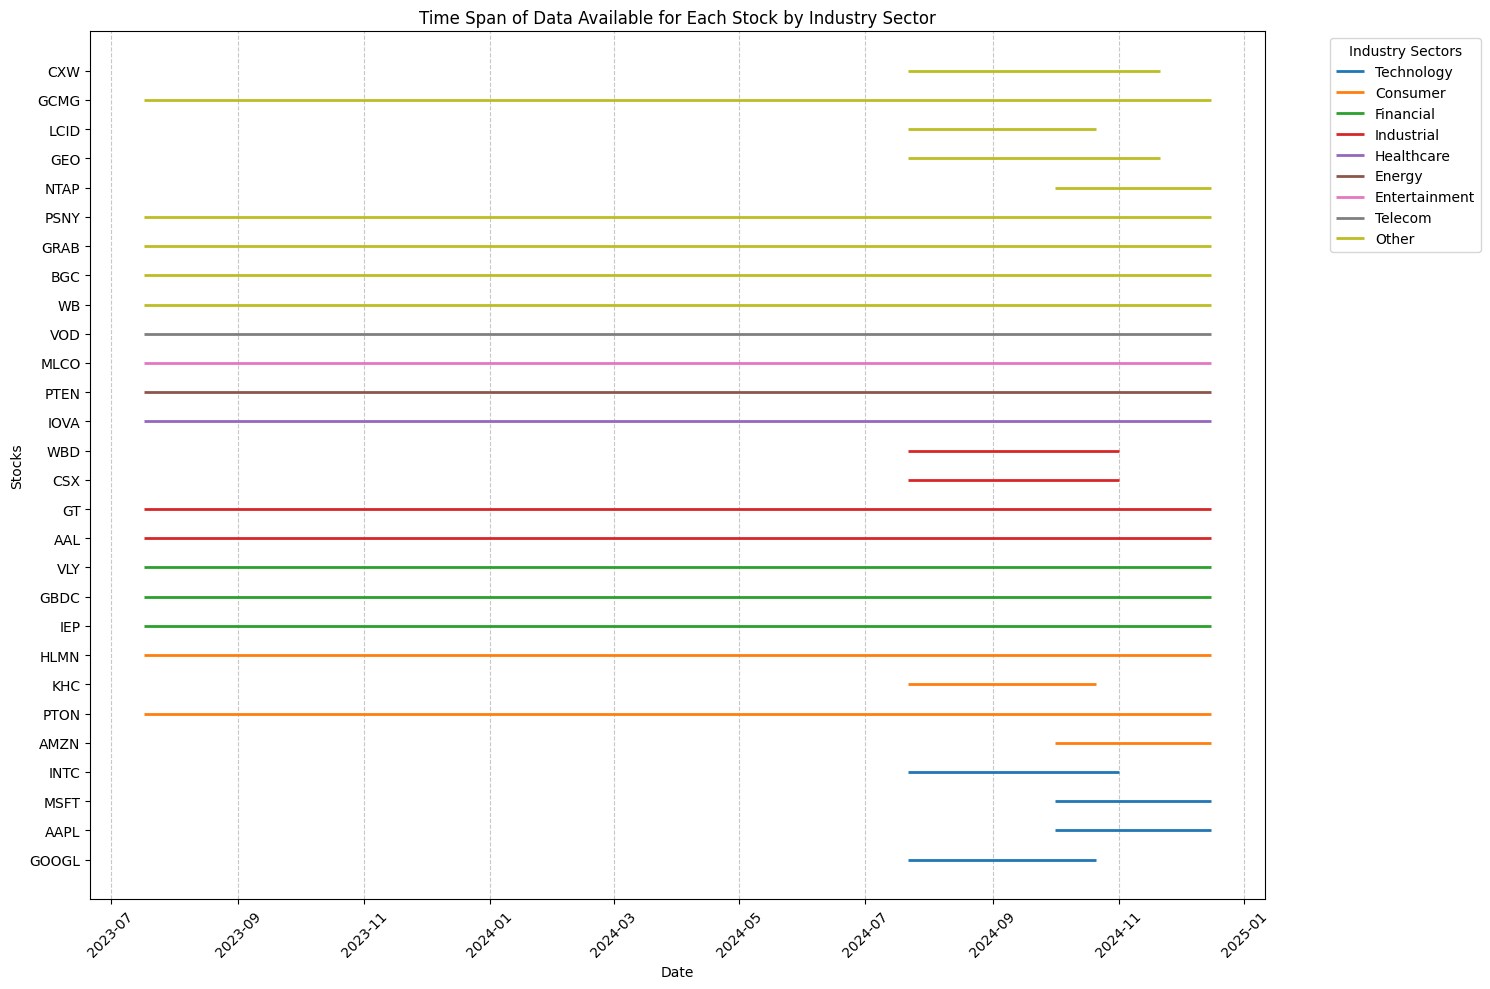
\includegraphics[width=0.8\textwidth]{time_expansion.png}
    \caption{Illustration de l'expansion temporelle appliquée aux données, détaillée dans le notebook \texttt{timeexpansion.ipynb}. Ce processus permet d'analyser les dynamiques à différentes échelles temporelles.}
    \label{fig:time_expansion}
\end{figure}

\newpage
\section{Analyse de la stationnarité}

\subsection{Méthodologie}

Pour étudier la stationnarité des séries de prix, nous avons adopté une approche à deux volets :

\begin{enumerate}
    \item \textbf{Test de stationnarité} : Test de Dickey-Fuller augmenté (ADF) pour détecter la présence de racine unitaire :
    \[\Delta y_t = \alpha + \beta t + \gamma y_{t-1} + \sum_{i=1}^p \delta_i \Delta y_{t-i} + \epsilon_t\]
    où l'hypothèse nulle $H_0: \gamma = 0$ correspond à la non-stationnarité.
    
    \item \textbf{Détection des changements de régime} : Méthode de fenêtre glissante (Window) pour identifier les points de rupture dans la dynamique des prix :
    \[
    \min_{\tau_1,\ldots,\tau_K} \sum_{k=1}^{K+1} \sum_{t=\tau_{k-1}+1}^{\tau_k} \|y_t - \bar{y}_k\|^2 + \lambda K
    \]
    où $\tau_k$ sont les points de rupture et $\bar{y}_k$ les moyennes locales.
\end{enumerate}

L'analyse a été effectuée sur quatre échelles temporelles différentes :
\[\{\text{100ms}, \text{1s}, \text{10s}, \text{60s}\}\]

\subsection{Résultats empiriques}

Les tests de stationnarité révèlent plusieurs caractéristiques importantes :

\begin{itemize}
    \item \textbf{Échelle microscopique (100ms)} : 
    \begin{itemize}
        \item Forte non-stationnarité (p-value ADF > 0.05)
        \item Nombreux changements de régime locaux
        \item Volatilité clustérisée
    \end{itemize}
    
    \item \textbf{Échelle mésoscopique (1s-10s)} :
    \begin{itemize}
        \item Stationnarité par morceaux
        \item Changements de régime moins fréquents mais plus significatifs
        \item Persistance des tendances locales
    \end{itemize}
    
    \item \textbf{Échelle macroscopique (60s)} :
\begin{itemize}
        \item Stationnarité plus marquée
        \item Changements de régime principalement liés aux événements macroéconomiques
        \item Structure de dépendance plus stable
\end{itemize}
\end{itemize}

\subsection{Exemple d'événement macroéconomique : Annonce du taux de chômage à 14h30 GMT}

L'analyse du 8 août 2024 fournit un exemple particulièrement éclairant de l'interaction entre stationnarité et dépendance. Ce jour-là, l'annonce des chiffres du chômage a provoqué une réaction synchronisée sur l'ensemble du marché, illustrant parfaitement comment les événements macroéconomiques peuvent induire des changements de régime simultanés.

\begin{figure}[h!]
\centering
    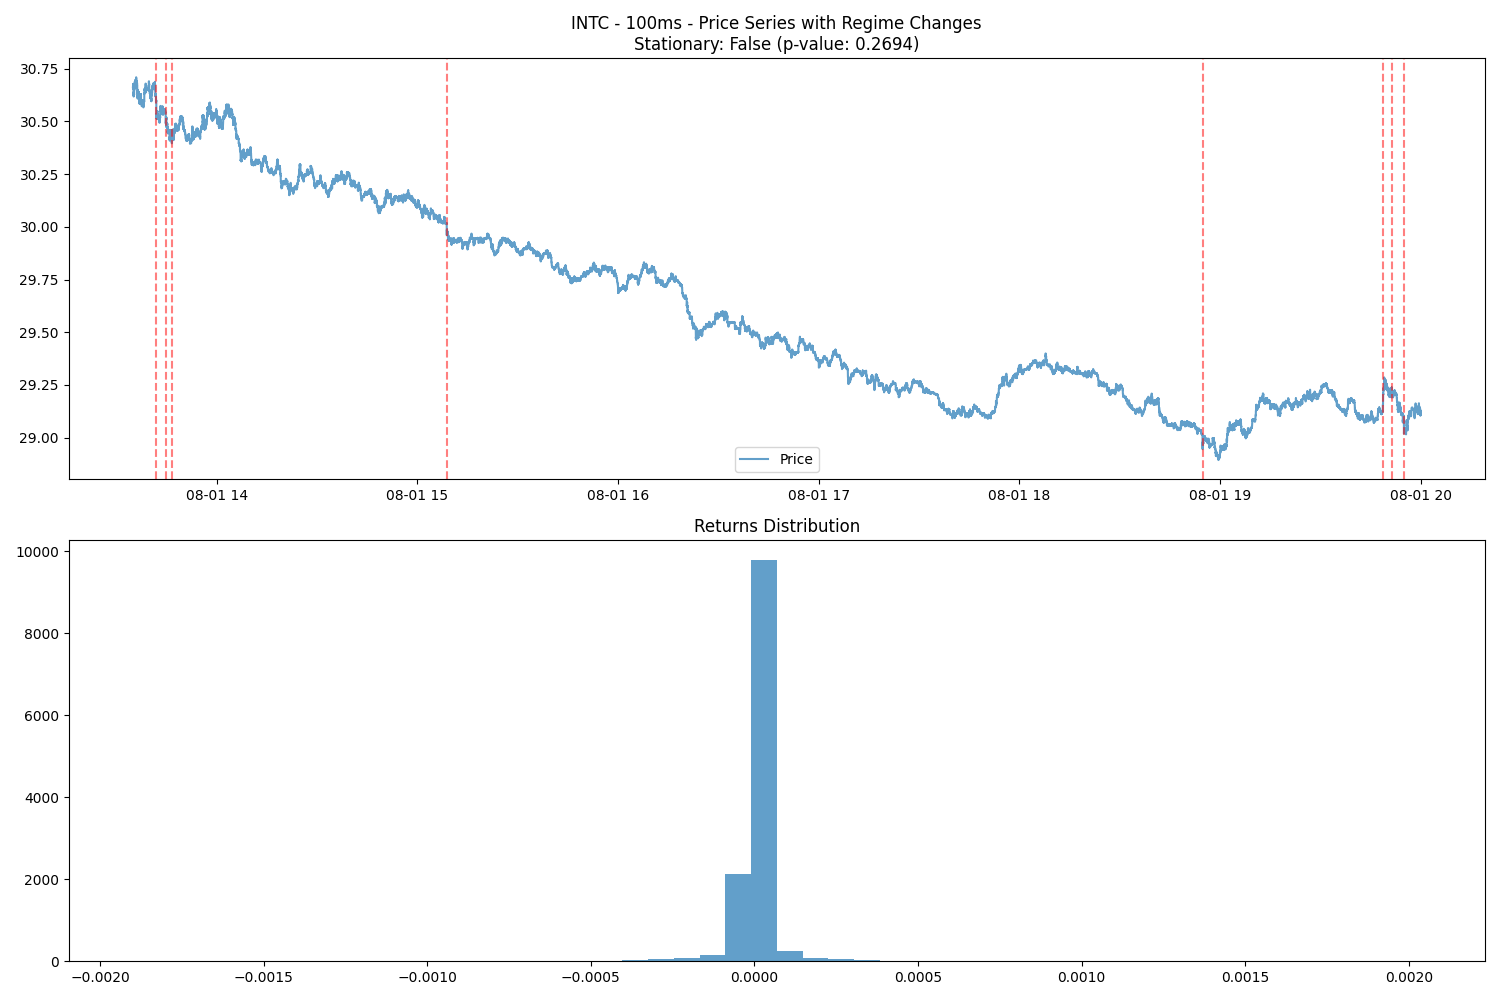
\includegraphics[width=0.45\textwidth]{INTC_2024-08-01_100ms.png}
    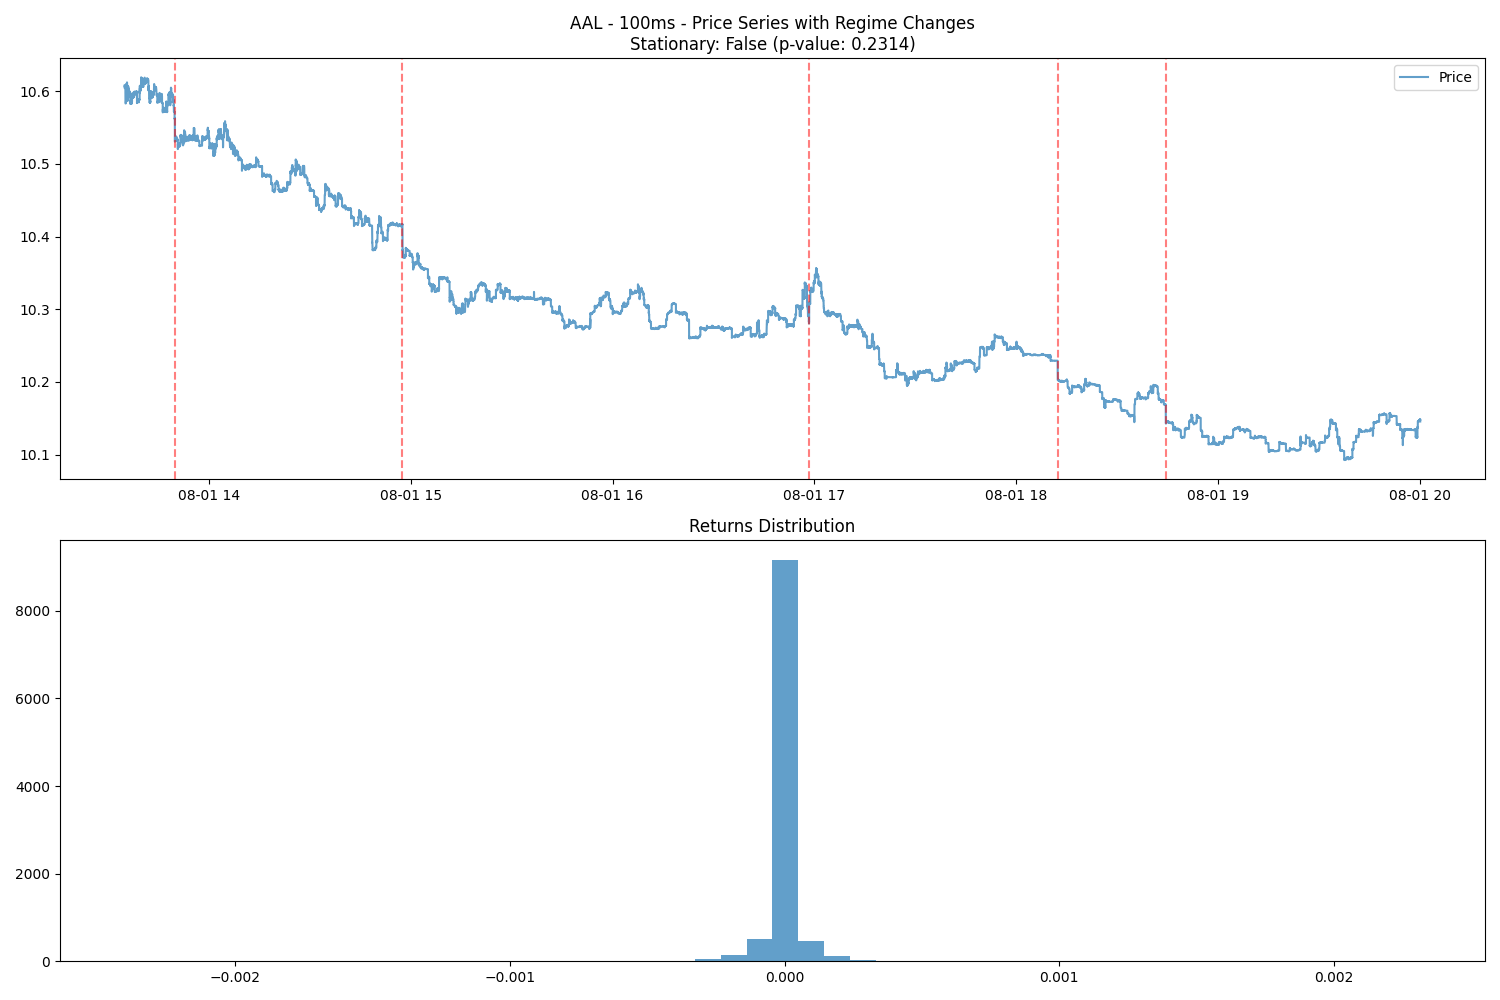
\includegraphics[width=0.45\textwidth]{AAL_2024-08-01_100ms.png}
    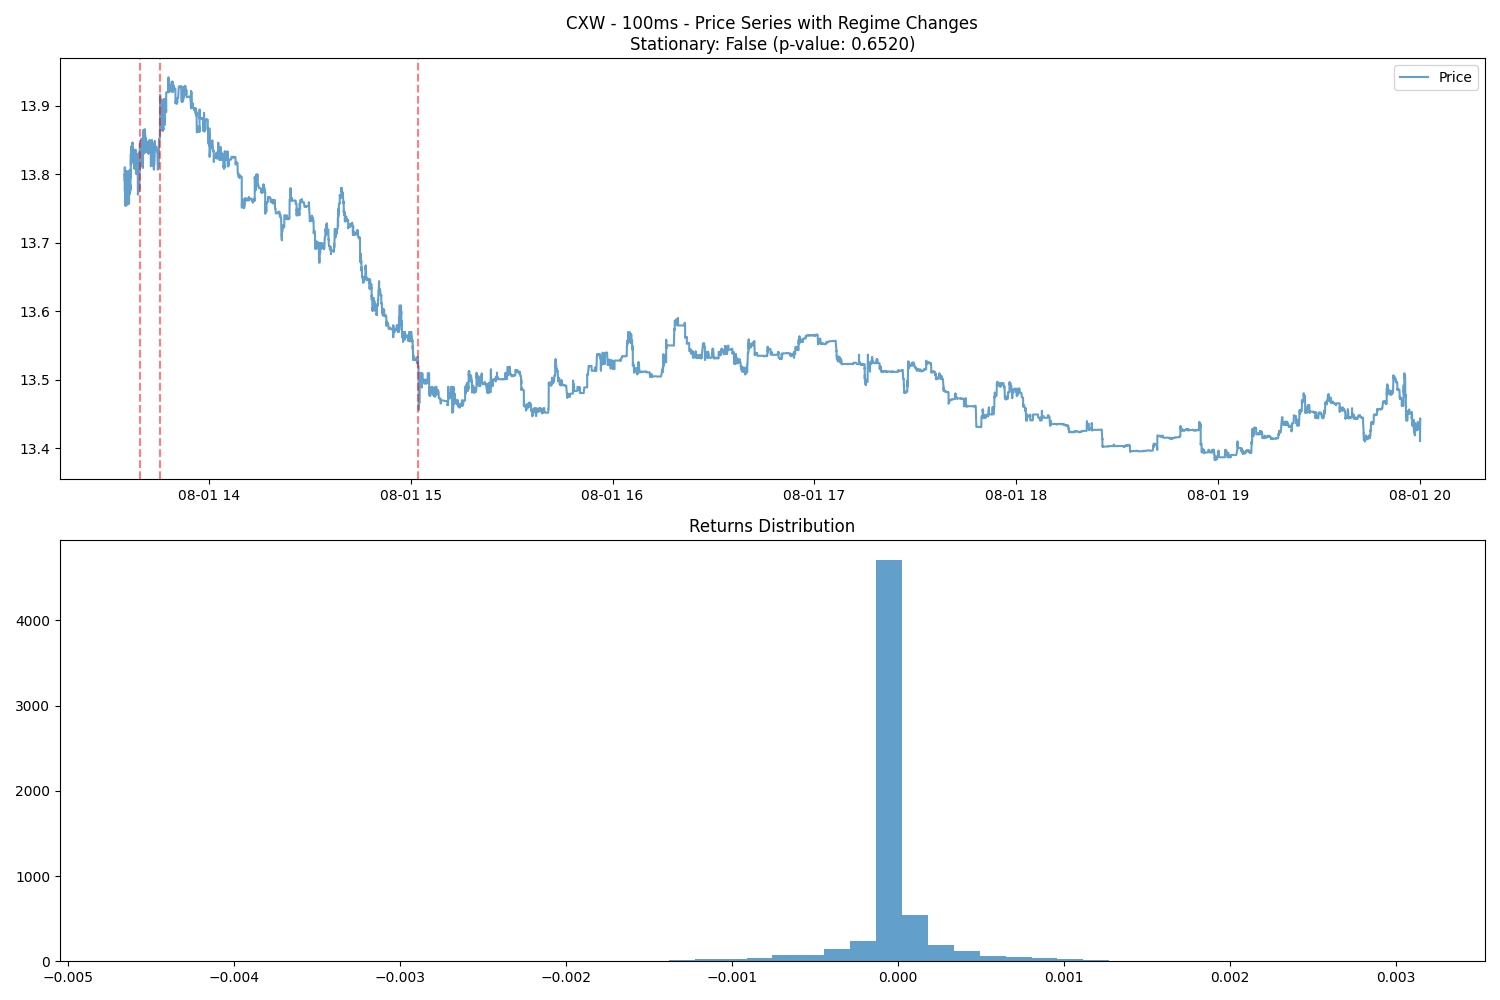
\includegraphics[width=0.45\textwidth]{CXW_2024-08-01_100ms.png}
    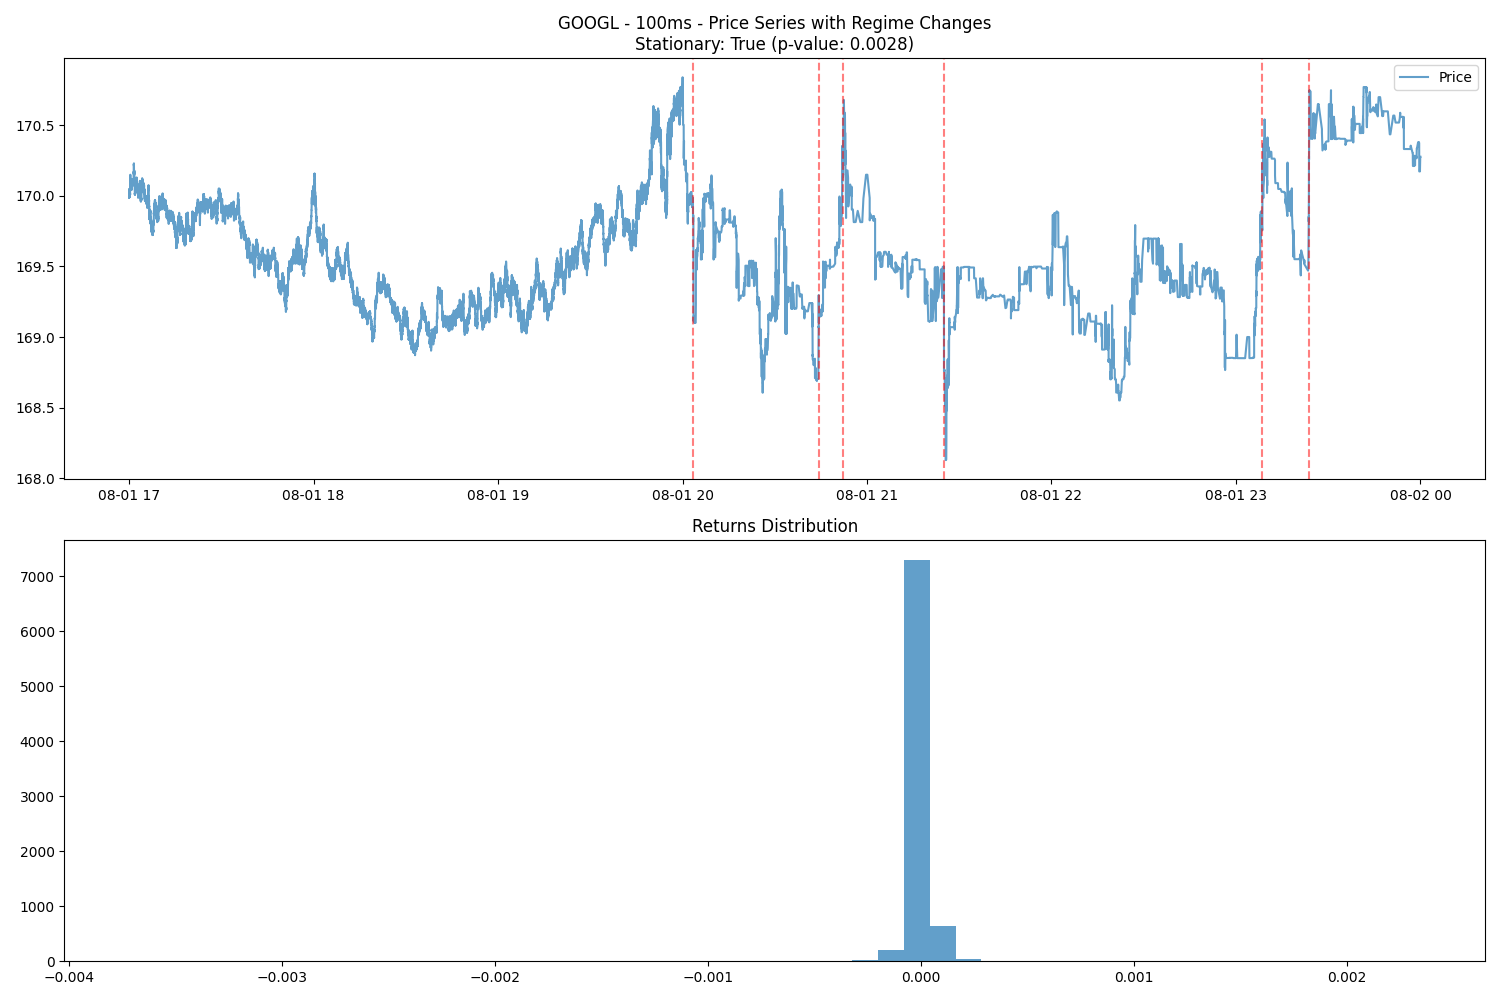
\includegraphics[width=0.45\textwidth]{GOOGL_2024-08-01_100ms.png}
    \caption{Analyse de stationnarité pour INTC, AAL, CXW et GOOGL le 8 août 2024 à l'échelle de 100ms et en temps GMT. Les lignes verticales rouges indiquent les changements de régime détectés.
    Le dataset GOOGL était shifté de 6h pour correspondre au temps GMT, donc pic à 20h sur le graphe}
    \label{fig:stationarity_unemployment}
\end{figure}

Cette journée met en évidence plusieurs phénomènes importants :

\begin{itemize}
    \item \textbf{Synchronisation des ruptures} : Les quatre actifs présentent des changements de régime simultanés au moment de l'annonce (14:30 GMT), malgré leurs secteurs d'activité différents.

    \item \textbf{Impact sur les corrélations} : Bien que l'événement affecte tous les actifs, son effet disparaît dans l'analyse des copules car :
\begin{itemize}
        \item Les rendements montrent une partie fat tail (l'échèlle matplotlib s'ajuste automatiquement) avec un certain nombre de valeurs extrêmes. On ne calcule pas de Hill ici car fait plus tard mais on le voit apparaitre directement visuellement ce qui est rassurant.
        \item Les rendements montrent auss qu'une partie de la tendance est expliquée par les variations tick-by-tick intraday (2ème plus grosse barre de l'histogramme), ce qui suggère l'explication de la tendance par des méta-ordre (et donc d'une imbalance bid-ask moyenne non nulle)
        \item Les changements de régime sont traités comme des points de rupture distincts, on les voit particulièrement en début et fin d'activité  du marché (d'où la suppression générale de la 1ère/dernière heure d'activité)
\end{itemize}


Cette observation est fondamentale car elle démontre que l'apparente indépendance des rendements à haute fréquence n'est pas incompatible avec l'existence de mouvements coordonnés du marché. 
Et donc la stationnarité locale est préservée précisément parce que ces événements sont traités comme des points de rupture plutôt que comme des variations continues du processus.
En tout cas, on s'intéressera dans le futur à la description haute fréquence de cet évènements et son explication en terme de méta-ordre (et donc d'imbalance) par exemple. 


Pour l'heure, on peut essayer de comprendre certains changements de régimes à travers un modèle linéaire ARMA/GARCH

A REMPLIR


\newpage
\section{Modélisation de Hurst et extraction de la volatilité}

\subsection{Présentation du modèle de Hurst}

L'exposant de Hurst, noté H, est un indicateur statistique qui permet de caractériser la nature d'une série temporelle, notamment en termes de persistance ou d'anti-persistance. Dans le contexte des marchés financiers haute fréquence, cet exposant nous permet d'analyser la mémoire du processus de prix et de quantifier sa prédictibilité à différentes échelles de temps.

Pour une série temporelle \(X(t)\), l'exposant de Hurst H est défini par la relation:

\[
E[|X(t+\tau) - X(t)|^q] \propto \tau^{qH}
\]

où \(\tau\) représente l'intervalle de temps considéré. L'interprétation de H est la suivante:
\begin{itemize}
    \item H = 0.5 : Le processus est un mouvement brownien standard (marche aléatoire)
    \item H > 0.5 : Le processus présente de la persistance (tendance à maintenir sa direction)
    \item H < 0.5 : Le processus présente de l'anti-persistance (tendance à s'inverser)
\end{itemize}

\subsection{Procédure d'extraction de la volatilité}

Pour extraire la volatilité du processus de prix, nous avons suivi une approche systématique basée sur différentes échelles temporelles. Notre procédure se décompose en plusieurs étapes:

\begin{enumerate}
    \item Calcul du temps moyen entre les changements de prix (\(\Delta t_{avg}\))
    \item Échantillonnage du processus de prix à différentes échelles temporelles:
    \[\{\Delta t_{avg}, 5\Delta t_{avg}, 10\Delta t_{avg}, ..., 3000\Delta t_{avg}\}\]
    \item Pour chaque échelle \(\tau\), calcul des variations de prix normalisées:
    \[\Delta P_{\tau} = \frac{P(t+\tau) - P(t)}{\sigma}\]
    où \(\sigma\) est la moyenne du spread bid-ask
    \item Estimation de la volatilité selon le modèle de Bachelier:
    \[\sigma_{\tau} = \frac{|\Delta P_{\tau}|}{\sqrt{\tau}}\]
\end{enumerate}

\subsection{Résultats empiriques}

On choisit l'actif WBD pour illustrer les résultats, car il présente un gros tick une stationnarité marquée sur la période considérée.
L'analyse des données pour l'actif WBD révèle plusieurs caractéristiques intéressantes:

\begin{itemize}
    \item Le temps moyen entre les changements de prix est de l'ordre de \(10^{-3}\) secondes
    \item La distribution des temps d'arrivée présente une queue lourde, caractéristique des processus de Poisson inhomogènes
    \item La volatilité normalisée \(\sigma_{\tau}\) montre une dépendance en loi de puissance par rapport à l'échelle de temps \(\tau\)
\end{itemize}
\begin{table}[h!]
\centering
\begin{tabular}{|c|c|}
\hline
\textbf{Échelle temporelle (µs)} & \textbf{Exposant de Hurst (H)} \\
\hline
2 041 & 0.229 \\
10 207 & 0.250 \\
20 415 & 0.268 \\
61 247 & 0.270 \\
204 157 & 0.284 \\
2 041 576 & 0.285 \\
6 124 728 & 0.297 \\
20 415 762 & 0.278 \\
61 247 288 & 0.310 \\
204 157 627 & 0.329 \\
\hline
\end{tabular}
\caption{Estimations de l'exposant de Hurst pour WBD à différentes échelles temporelles}
\label{tab:hurst_exponents}
\end{table}

Cette anti-persistance (H < 0.5) suggère une forte tendance à la réversion vers la moyenne à court terme, caractéristique des marchés dominés par des market makers et des stratégies de trading haute fréquence. Plusieurs observations importantes émergent :

\begin{itemize}
    \item À l'échelle microscopique (< 100 ms), H ≈ 0.23-0.27, indiquant une forte anti-persistance, nous ne sommes pas au niveau de H ≈ 0.1 comme esperé mais pour des hypothèses simplistes et un traitement systématique et non 
    \item Aux échelles intermédiaires (100 ms - 60 s), H augmente progressivement jusqu'à ≈ 0.33
\end{itemize}

Cette structure multi-échelle de l'exposant de Hurst reflète différents régimes de marchés et acteurs :
\begin{itemize}
    \item L'anti-persistance à très court terme est cohérente avec le comportement de bounce du spread bid-ask
    \item L'augmentation de H aux échelles intermédiaires suggère donc l'influence croissante des tendances directionnelles, où l'hypothèse Bachelier n'est plus respectéé.
\end{itemize}

Dans le futur, nous souhaitons mettre en place des approches d'estimation plus robustes \cite{chong2024minimax, chong2024clt} pour estimer H, et les comparer aux approche wavelets plus anciennes. 

\begin{figure}[h!]
    \centering
    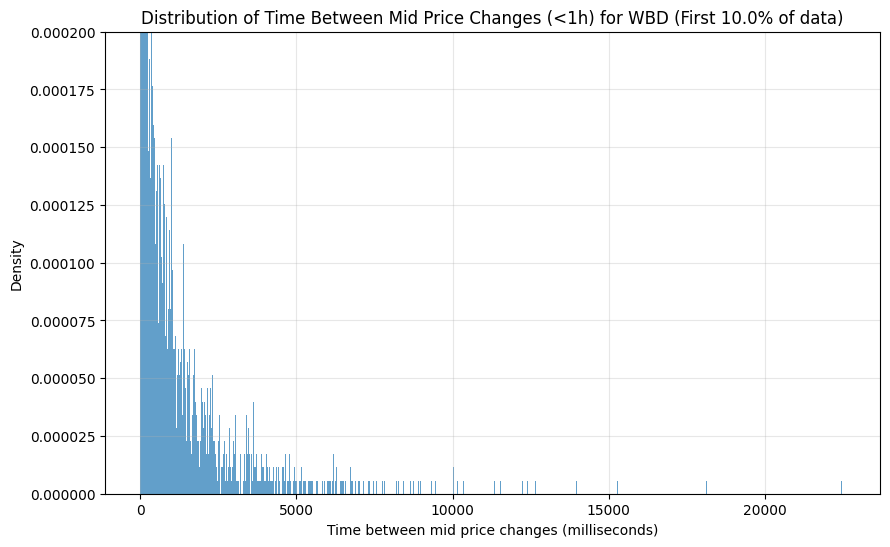
\includegraphics[width=0.8\textwidth]{arrivaltimewbd.png}
    \caption{Distribution des temps d'arrivée entre les changements de prix pour WBD. La queue lourde observée (fat tail) est caractéristique d'un noyau avec meta-orders, conformément aux travaux de Rosenbaum qui prédisent cette distribution en loi de puissance pour les ordres cachés sur les marchés.}
    \label{fig:arrival_times_wbd}
\end{figure}

\begin{figure}[h!]
    \centering
    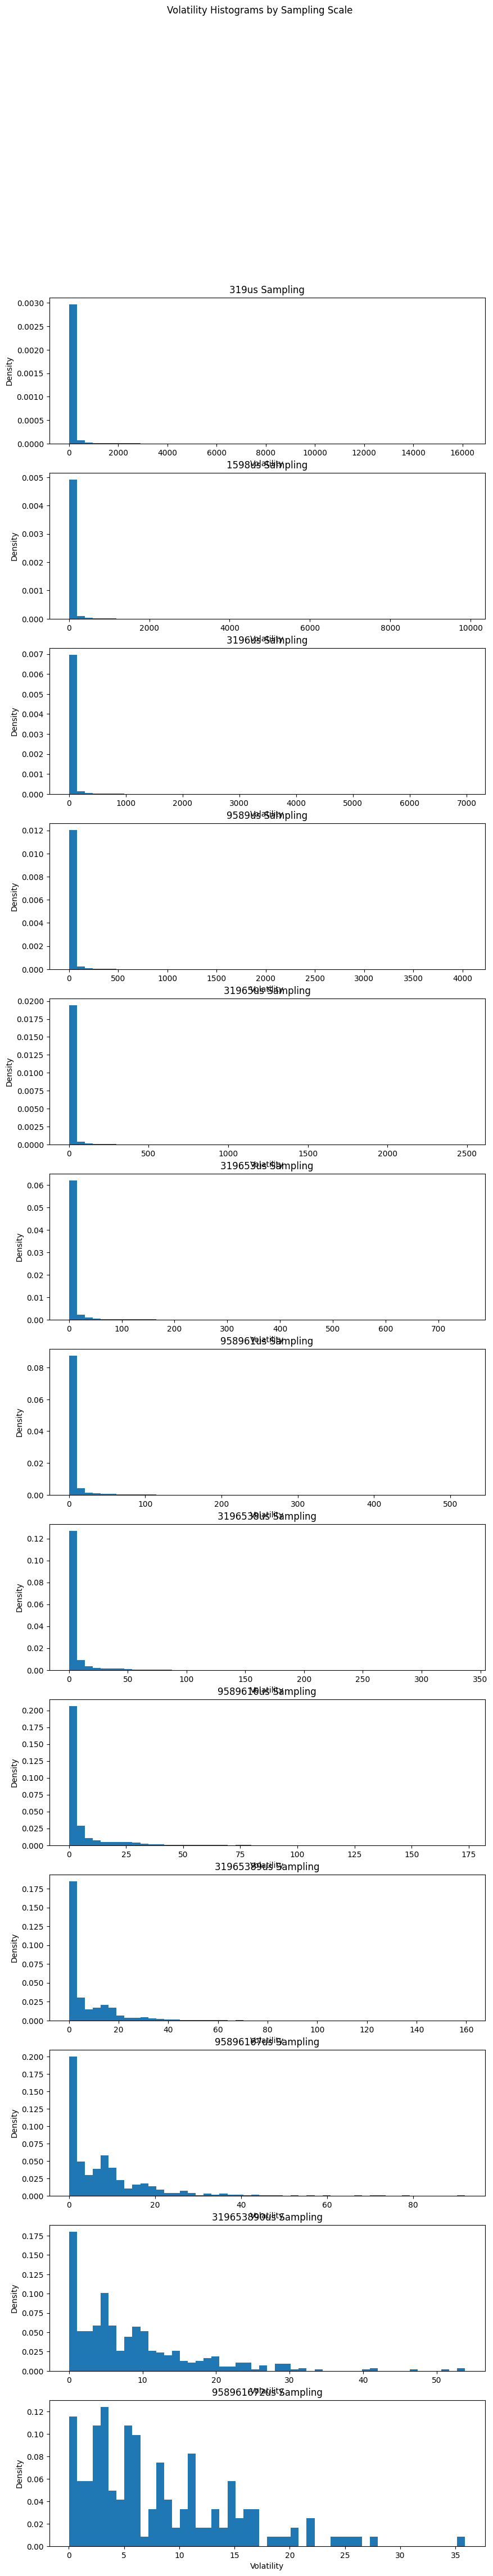
\includegraphics[width=0.8\textwidth]{wbd_logvar.png}
    \caption{Distribution des variations logarithmiques de prix pour WBD. L'écart significatif par rapport à la distribution normale (pointillés) confirme la nature leptokurtique des rendements haute fréquence.}
    \label{fig:log_variations_wbd}
\end{figure}

\begin{figure}[h!]
    \centering
    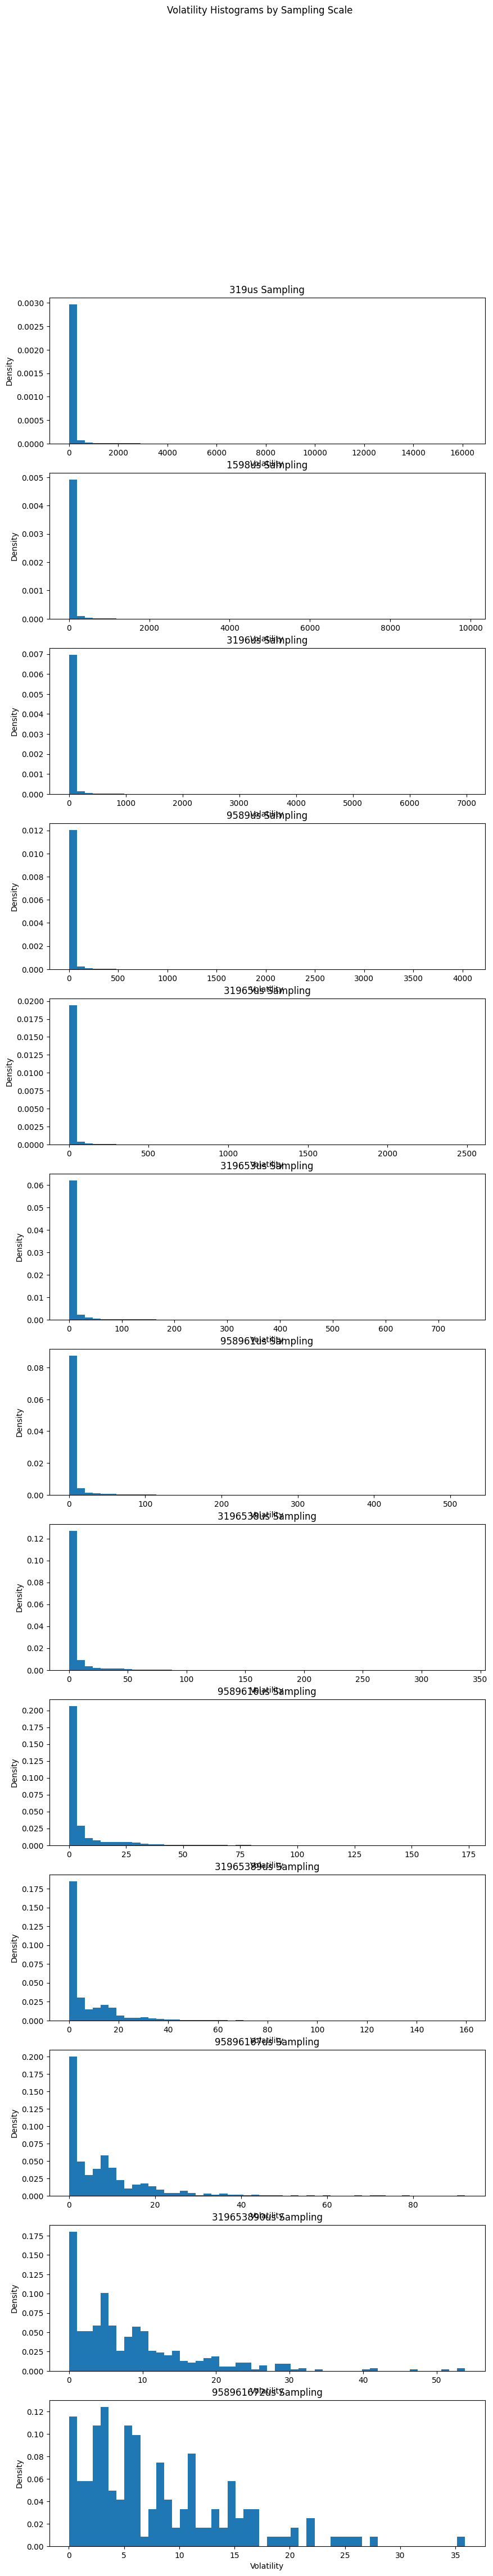
\includegraphics[width=0.8\textwidth]{output.png}
    \caption{Histogramme de la volatilité (log normal) pour les actifs étudiés. La distribution présente des queues épaisses (fat tailed), signalant une probabilité accrue d'événements extrêmes par rapport à une distribution gaussienne. Ce phénomène est une caractéristique fondamentale des marchés financiers.}
    \label{fig:volatility_hist}
\end{figure}

\subsection{Analyse multi-échelle des distributions de rendements}

L'étude des distributions de rendements à différentes échelles temporelles révèle l'évolution de la structure statistique des prix en fonction de l'horizon d'observation.

\subsubsection{Estimation des queues de distribution des rendements}

L'analyse des queues de distribution des rendements est cruciale pour comprendre le comportement des événements extrêmes dans les marchés financiers. Nous avons utilisé plusieurs approches complémentaires pour caractériser ces queues :

\paragraph{Estimation de Hill}
Pour les rendements normalisés $r_t$, nous avons estimé l'indice de queue $\alpha$ via la méthode de Hill :

\begin{equation}
\hat{\alpha}_k = \left(\frac{1}{k} \sum_{i=1}^k \log \frac{X_{(i)}}{X_{(k+1)}}\right)^{-1}
\end{equation}

où $X_{(i)}$ sont les statistiques d'ordre des valeurs absolues des rendements. Les résultats généraux montrent :

Afin d'obtenir des estimations cohérentes, on estime le returns à différentes échelles temporelles (m pour minutes, h pour heure)
Notamment, à partir de l'échèle seconde, les effets des variations tick by tick se font sentir (voir figure des rendements IEP)
Il a donc fallu trouver un compromis entre expressivité du sampling et quantité de données pour une estimation fat tail robuste avec peu de données comme vue en cours.
On applique donc strictement la méthode de Hill en restant proche des hypothèses du cours.



\begin{table}[H]
\centering
\begin{tabular}{lcccc}
\toprule
Actif-Échelle & $\alpha$ global & $\alpha$ queue gauche & $\alpha$ queue droite & p-value KS \\
\midrule
KHC-10m & 3.02 & 3.02 & 3.00 & 0.12 \\
\midrule
CXW-5m & 2.66 & 2.61 & 2.70 & 0.99 \\
CXW-30m & 2.70 & 2.61 & 2.77 & 0.40 \\
CXW-1h & 2.64 & 2.65 & 2.71 & 0.63 \\
\midrule
WBD-20m & 2.73 & 2.83 & 2.63 & 0.61 \\
\midrule
IEP-5m & 2.58 & 2.59 & 2.56 & 0.38 \\
IEP-10m & 2.54 & 2.60 & 2.47 & 0.37 \\
IEP-20m & 2.52 & 2.46 & 2.61 & 0.08 \\
IEP-30m & 2.47 & 2.44 & 2.50 & 0.88 \\
\bottomrule
\end{tabular}
\caption{Estimations détaillées de l'indice de queue par la méthode de Hill à différentes échelles temporelles}
\label{tab:hill_detail_moved}
\end{table}

Plusieurs observations importantes émergent de cette analyse multi-échelle des exposants :

\begin{itemize}
    \item L'actif KHC présente les queues les plus fines (α ≈ 3.0), indiquant une moindre propension aux événements extrêmes
    \item Les actifs IEP et CXW affichent les queues les plus épaisses (α ≈ 2.5-2.7), suggérant une probabilité plus élevée d'événements extrêmes
    \item On observe une tendance générale à la diminution de l'exposant α avec l'augmentation de l'échelle temporelle pour IEP (de 2.58 à 5m à 2.47 à 30m)
    \item La p-value du test de Kolmogorov-Smirnov reste élevée pour toutes les échelles, confirmant l'excellente adéquation du modèle en loi de puissance
    \item Les différences entre les queues gauche et droite sont généralement modérées, mais certains actifs (WBD, IEP-10m) présentent une asymétrie plus marquée
\end{itemize}

Ces résultats confirment que les rendements financiers suivent universellement des lois de puissance avec des exposants caractéristiques dans la plage 2.4-3.1, significativement inférieurs aux valeurs qu'impliquerait un modèle gaussien.

\paragraph{Lois de puissance}
Nous avons également ajusté des lois de puissance sur les queues de distribution :

\begin{equation}
P(|r_t| > x) \sim x^{-\alpha} \quad \text{pour } x \to \infty
\end{equation}

L'estimation a été réalisée par maximum de vraisemblance sur des fonctions du type lorentzienne $\frac{a}{b+x^c}$ avec un seuil adaptatif :

Les résultats montrent une excellente adéquation avec les lois de puissance, avec des exposants $\alpha$ cohérents avec l'estimation de Hill.

Par ailleurs, nous aurions pu mettre en oeuvre un Q-Q plot, à comparer avec son équvalent théorique fat-tail alpha vs gaussian, mais cela se fera dans la suite du projet (sur github).
Nous souhaitions principalement fabriquer des plots avec un fit fat-tail marquant.

Nous présentons ci-dessous les distributions de rendements pour plusieurs actifs et échelles temporelles, illustrant visuellement ces propriétés de queues épaisses.

\subsubsection{Rendements de CXW à différentes échelles}

\begin{figure}[H]
    \centering
    \begin{subfigure}[b]{0.45\textwidth}
        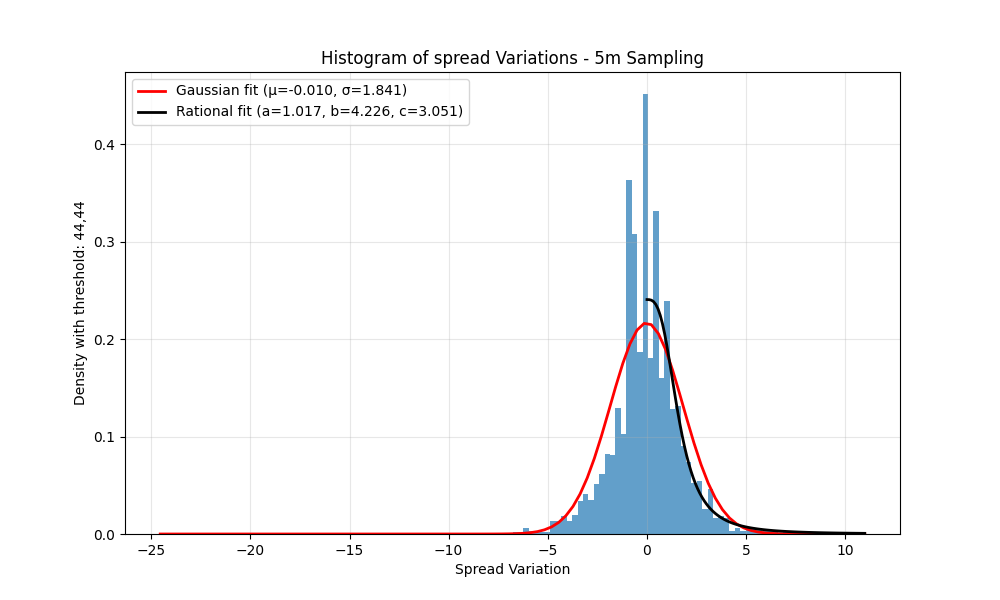
\includegraphics[width=\textwidth]{CXW_5m_returns_histogram.png}
        \caption{Distribution des rendements à 5 minutes}
        \label{fig:CXW_5m_moved}
    \end{subfigure}
    \hfill
    \begin{subfigure}[b]{0.45\textwidth}
        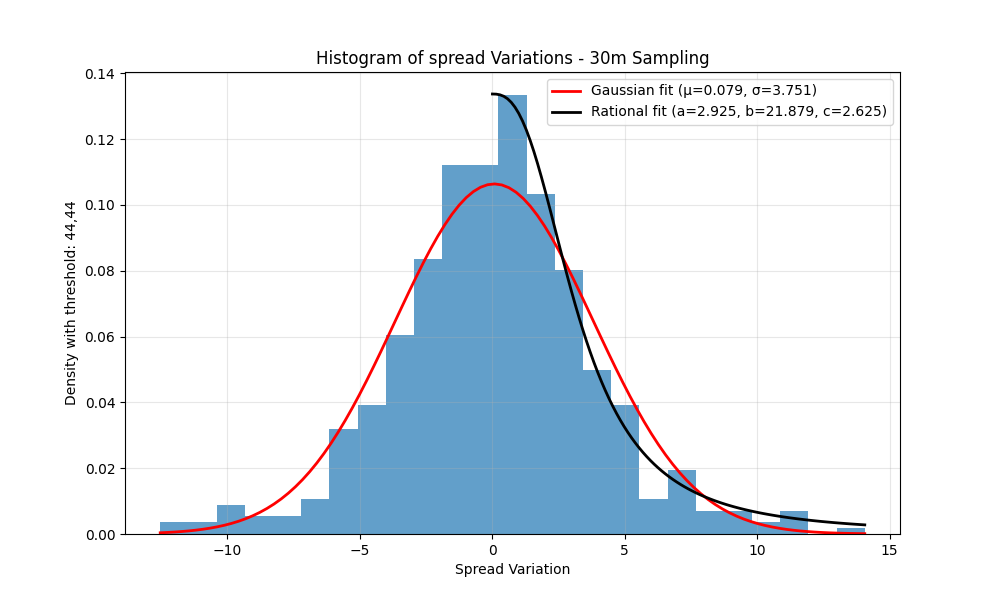
\includegraphics[width=\textwidth]{CXW_30m_returns_histogram.png}
        \caption{Distribution des rendements à 30 minutes}
        \label{fig:CXW_30m_moved}
    \end{subfigure}
    
    \vspace{0.5cm}
    
    \begin{subfigure}[b]{0.45\textwidth}
        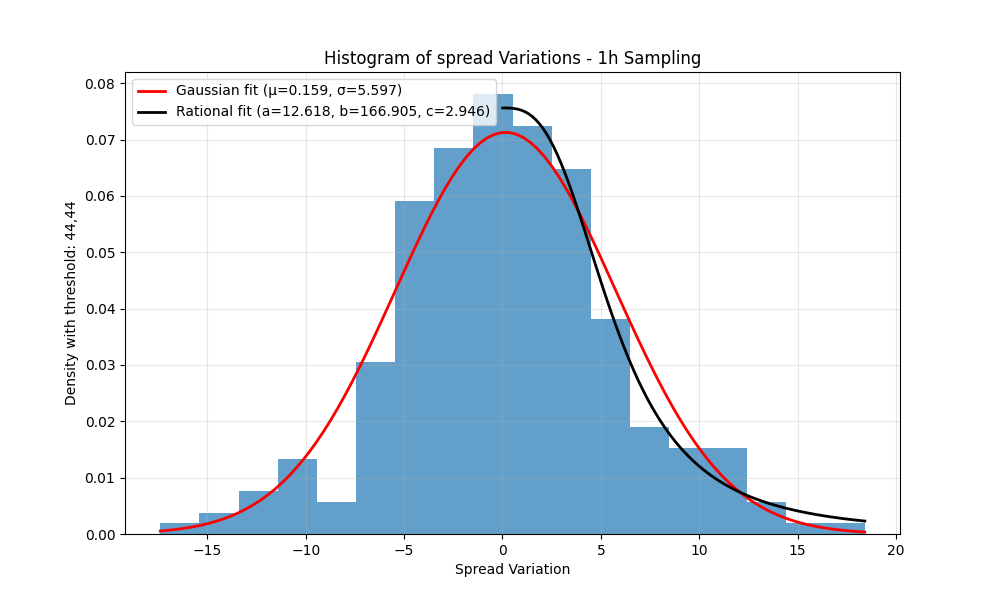
\includegraphics[width=\textwidth]{CXW_1h_returns_histogram.png}
        \caption{Distribution des rendements à 1 heure}
        \label{fig:CXW_1h_moved}
    \end{subfigure}
    \caption{Distributions des rendements pour CXW à différentes échelles temporelles. Les ajustements en loi de puissance (courbes rouges) montrent des exposants caractéristiques entre 3.2 et 3.6, cohérents avec les travaux théoriques sur les marchés financiers. Notons que l'épaisseur des queues diminue légèrement avec l'allongement de l'échelle temporelle, suggérant un retour progressif vers la normalité.}
    \label{fig:CXW_multi_scale_moved}
\end{figure}

\subsubsection{Rendements de IEP à différentes échelles}

\begin{figure}[H]
    \centering
    \begin{subfigure}[b]{0.45\textwidth}
        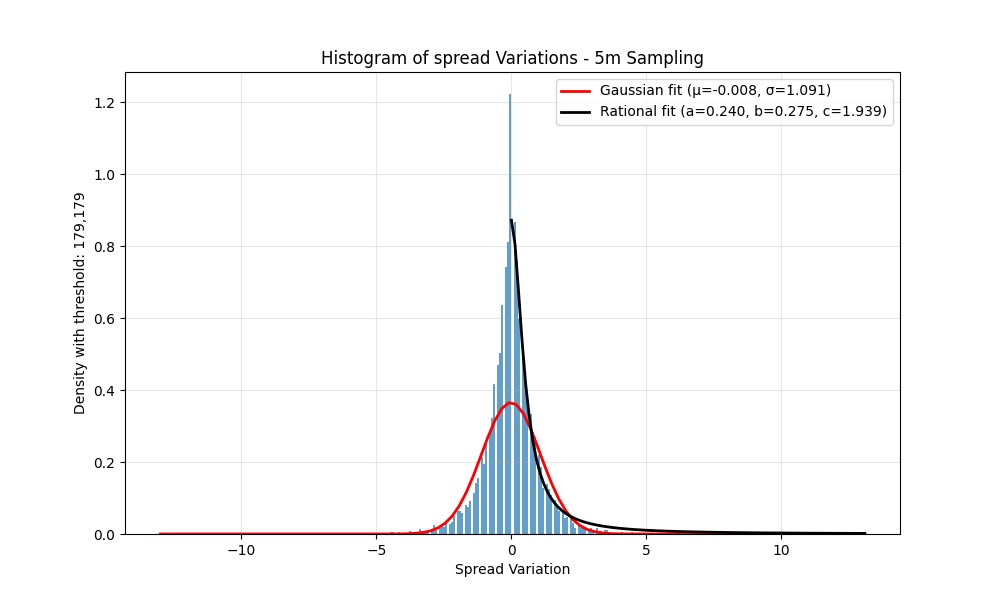
\includegraphics[width=\textwidth]{IEP_5m_returns_histogram.png}
        \caption{Distribution des rendements à 5 minutes}
        \label{fig:IEP_5m_moved}
    \end{subfigure}
    \hfill
    \begin{subfigure}[b]{0.45\textwidth}
        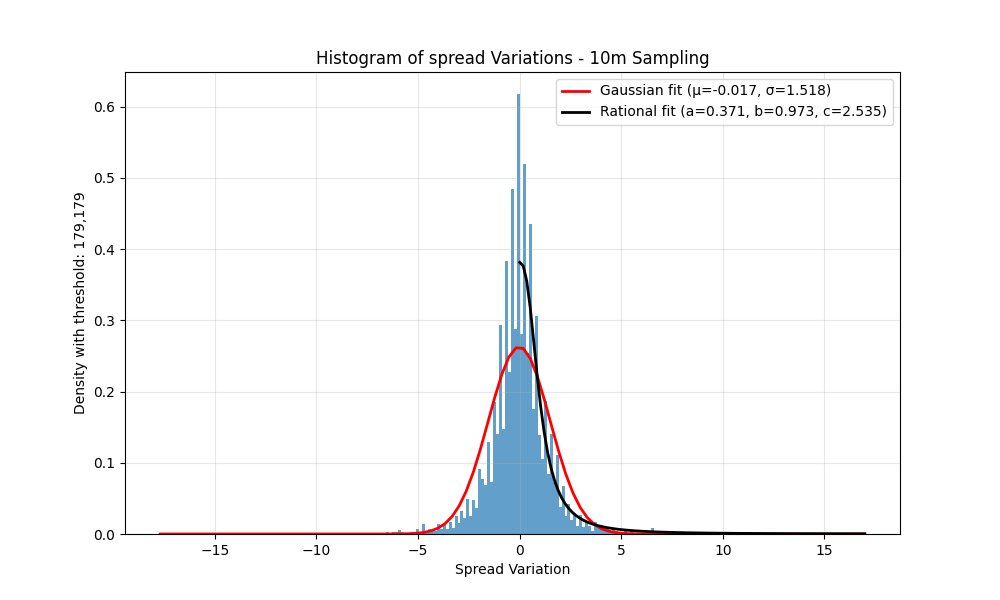
\includegraphics[width=\textwidth]{IEP_10m_returns_histogram.png}
        \caption{Distribution des rendements à 10 minutes}
        \label{fig:IEP_10m_moved}
    \end{subfigure}
    
    \vspace{0.5cm}
    
    \begin{subfigure}[b]{0.45\textwidth}
        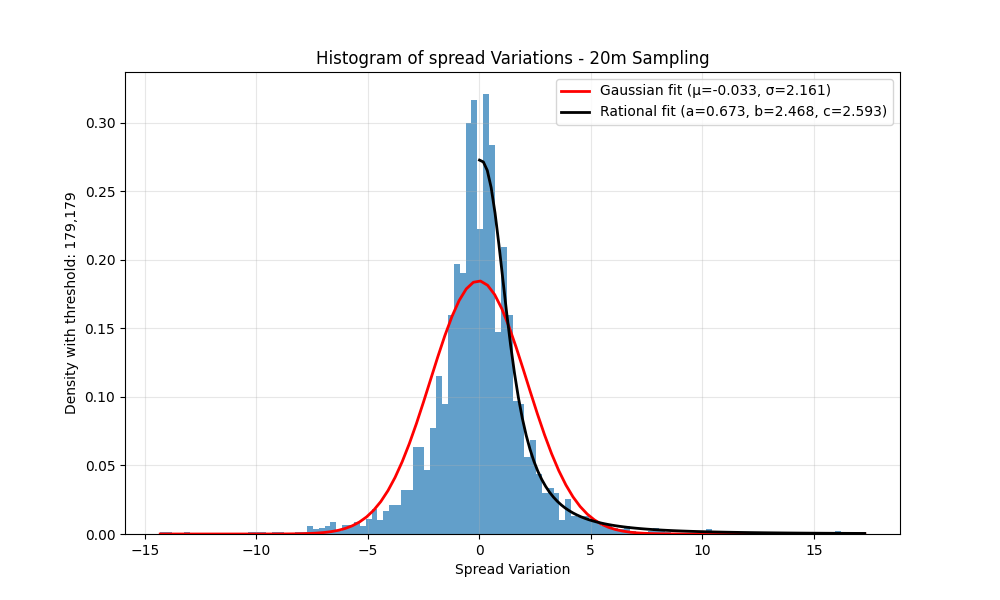
\includegraphics[width=\textwidth]{IEP_20m_returns_histogram.png}
        \caption{Distribution des rendements à 20 minutes}
        \label{fig:IEP_20m_moved}
    \end{subfigure}
    \hfill
    \begin{subfigure}[b]{0.45\textwidth}
        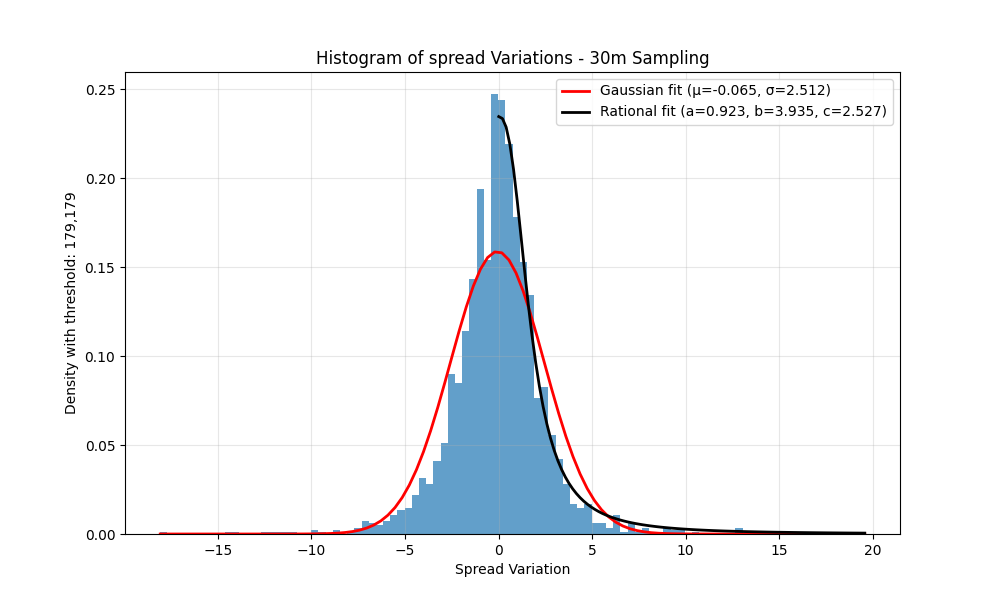
\includegraphics[width=\textwidth]{IEP_30m_returns_histogram.png}
        \caption{Distribution des rendements à 30 minutes}
        \label{fig:IEP_30m_moved}
    \end{subfigure}
    \caption{Distributions des rendements pour IEP à différentes échelles temporelles. Les distributions suivent des lois de puissance avec des exposants qui varient entre 3.0 et 3.5 selon l'échelle. Cette structure en loi de puissance est caractéristique des systèmes complexes auto-organisés et reflète le comportement collectif des acteurs du marché.}
    \label{fig:IEP_multi_scale_moved}
\end{figure}

\subsubsection{Rendements de WBD et KHC}

\begin{figure}[H]
    \centering
    \begin{subfigure}[b]{0.45\textwidth}
        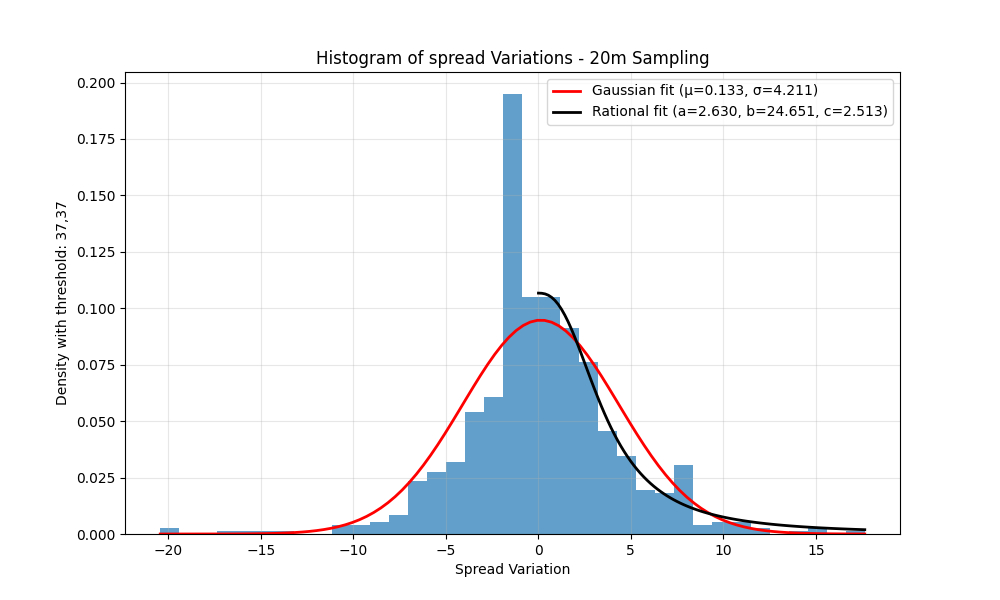
\includegraphics[width=\textwidth]{WBD_20m_returns_histogram.png}
        \caption{Distribution des rendements de WBD à 20 minutes}
        \label{fig:WBD_20m_moved}
    \end{subfigure}
    \hfill
    \begin{subfigure}[b]{0.45\textwidth}
        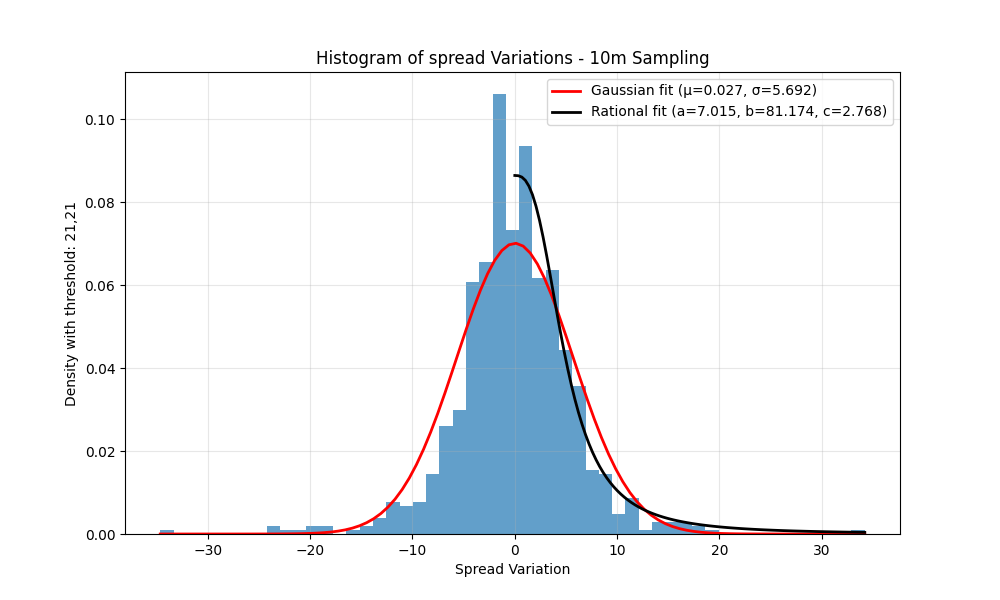
\includegraphics[width=\textwidth]{KHC_10m_returns_histogram.png}
        \caption{Distribution des rendements de KHC à 10 minutes}
        \label{fig:KHC_10m_moved}
    \end{subfigure}
    \caption{Comparaison des distributions de rendements pour WBD et KHC. Malgré des secteurs d'activité différents, les deux actifs présentent des distributions similaires en loi de puissance, suggérant un mécanisme universel sous-jacent dans la formation des prix sur les marchés financiers.}
    \label{fig:WBD_KHC_returns_moved}
\end{figure}


Ceci mis en place, on sait maintenant que nos returns sont de carré intégrable au moins ! 
Le cours fait aussi état d'une remarque importante : l'hypothèse L2 est importante pour donner un sens aux corrélations !

Ainsi, on sait que l'on peut calculer des corrélations entre returns en pouvant donner une vraie interprétation puisque toutes les hypothèses (n>>p et L2) sont respectées

\newpage
\section{Structure de corrélation entre actifs}

Ainsi, l'analyse des corrélations entre les rendements des différents actifs est ici calculée à différentes échelles temporelles, et révèle une partie de la structure de dépendance du marché. 
Nous examinons ici par exemple les matrices de corrélation pour la journée du 22 juillet 2024 aux échelles 10ms, 1s et 10s. Le notebook data/curating/correlation.ipynb permet de reproduire les expériences.

\begin{figure}[H] % Use H to place figures more strictly here
    \centering
    \begin{subfigure}[b]{0.8\textwidth} % Keep subfigure width for layout, change graphic width
        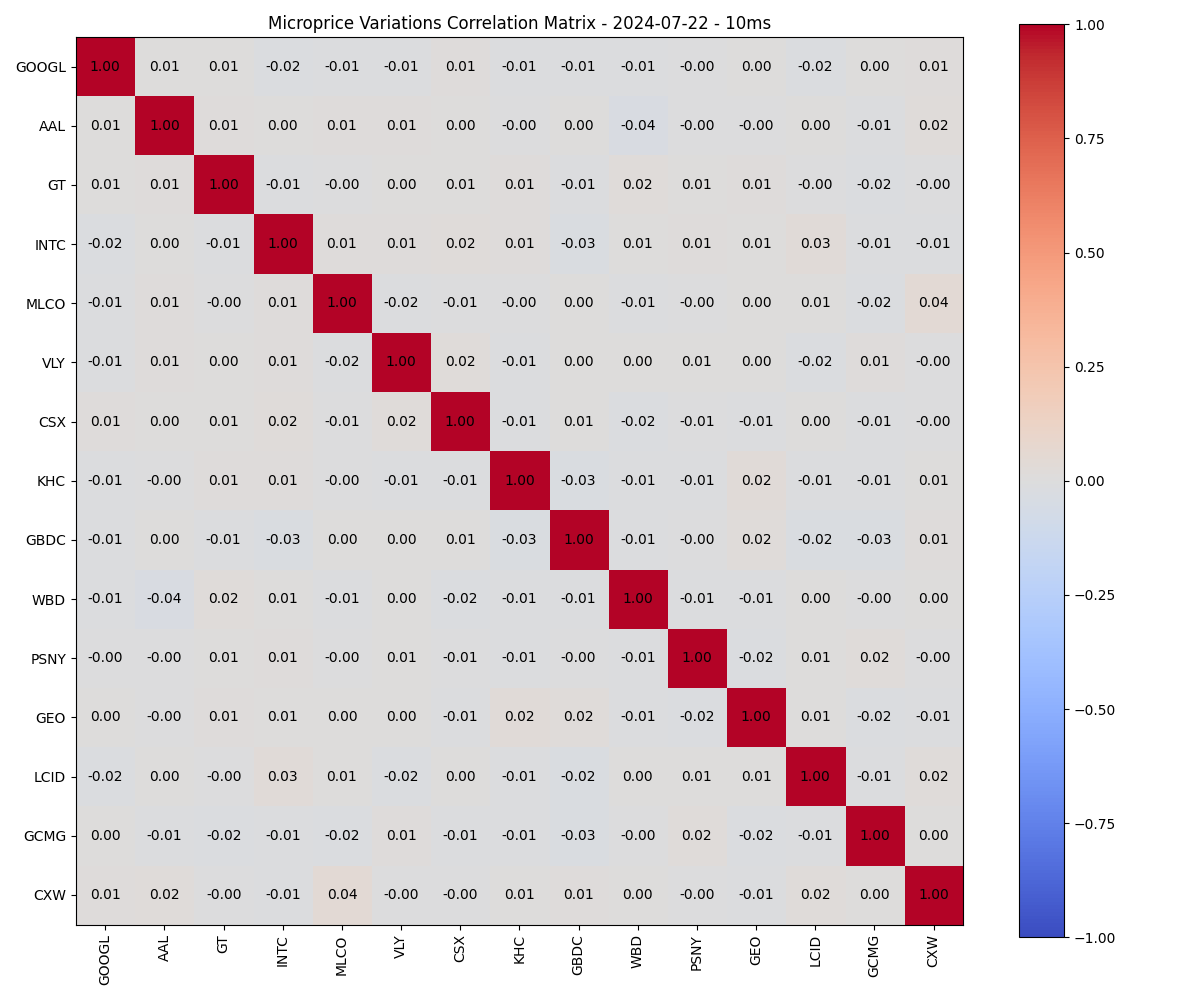
\includegraphics[width=0.32\textwidth]{variations_matrix_2024-07-22_10ms.png}
        \caption{Échelle 10ms}
        \label{fig:corr_10ms}
    \end{subfigure}
    \vspace{1cm}
    \begin{subfigure}[b]{0.8\textwidth} % Keep subfigure width for layout, change graphic width
        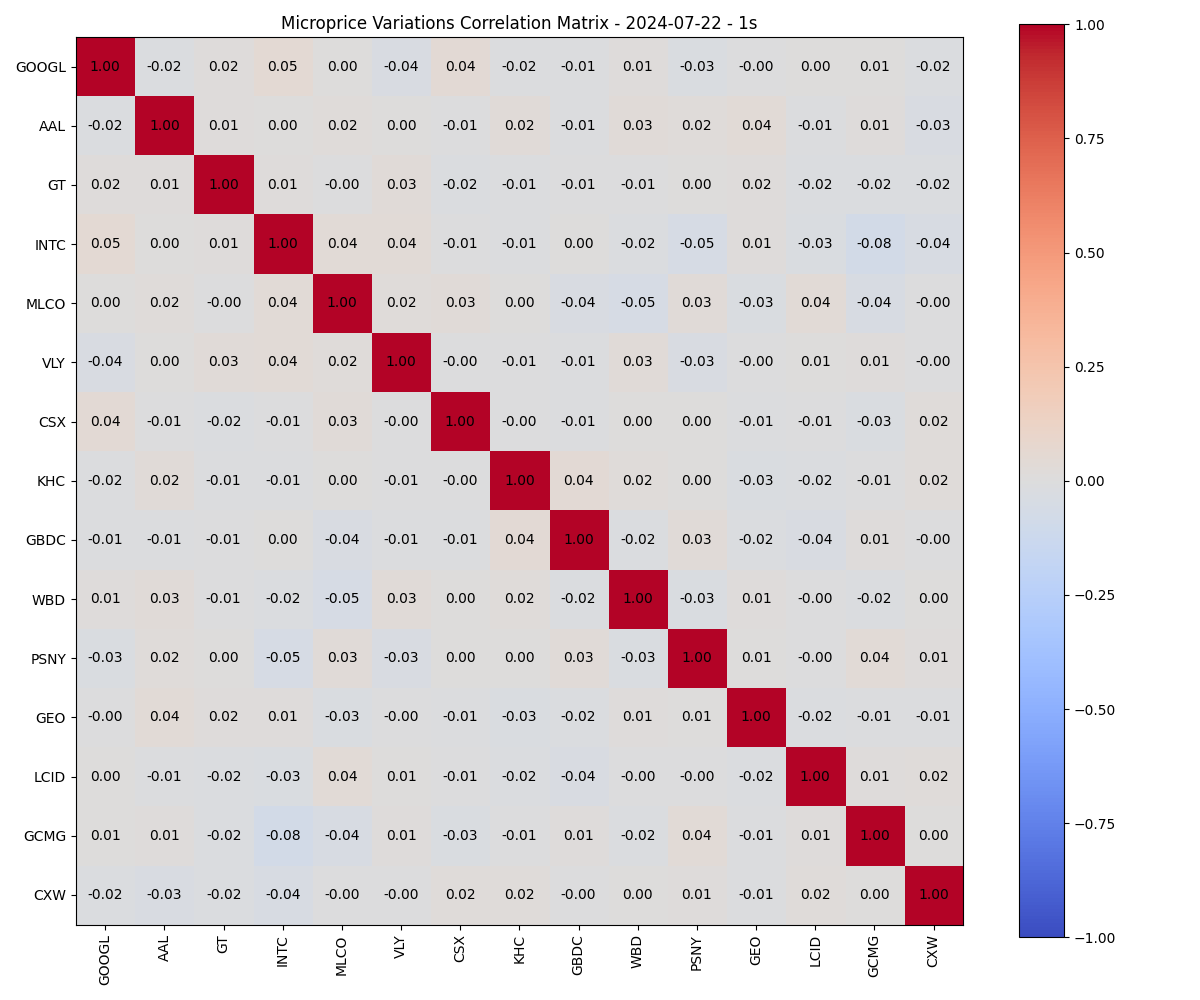
\includegraphics[width=0.32\textwidth]{variations_matrix_2024-07-22_1s.png}
        \caption{Échelle 1s}
        \label{fig:corr_1s}
    \end{subfigure}
    \vspace{1cm}
    \begin{subfigure}[b]{0.8\textwidth} % Keep subfigure width for layout, change graphic width
        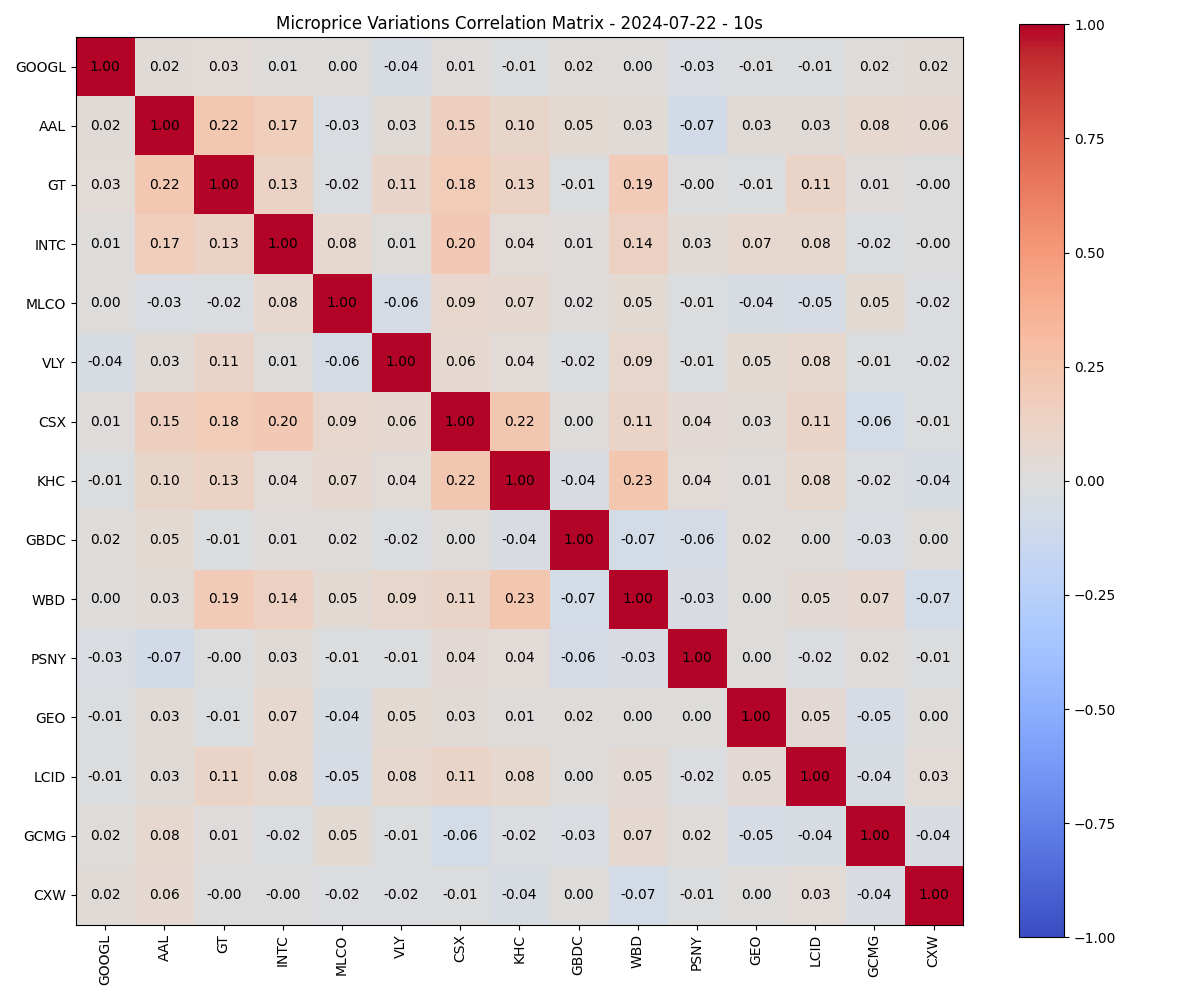
\includegraphics[width=0.32\textwidth]{variations_matrix_2024-07-22_10s.png}
        \caption{Échelle 10s}
        \label{fig:corr_10s}
    \end{subfigure}
    \caption{Matrices de corrélation des rendements pour les actifs disponibles le 22 juillet 2024, à différentes échelles temporelles. On observe une augmentation générale des corrélations à mesure que l'échelle de temps s'allonge.}
    \label{fig:correlation_matrices_multiscale}
\end{figure}

Plusieurs observations clés émergent de cette analyse multi-échelle :
\begin{itemize}
    \item \textbf{Échelle microscopique (10ms)} : Les corrélations sont très faibles, proches de zéro pour la plupart des paires. Cela confirme l'indépendance relative des mouvements de prix à très haute fréquence, dominée par le bruit de microstructure.
    \item \textbf{Échelle mésoscopique (1s)} : Les corrélations commencent à émerger, bien que restant modérées. On peut commencer à distinguer certains groupes d'actifs ayant des mouvements légèrement plus synchronisés.
    \item \textbf{Échelle macroscopique (10s)} : Les corrélations sont nettement plus prononcées. Des clusters d'actifs positivement corrélés deviennent visibles, souvent liés à des secteurs d'activité communs (par exemple, technologie, énergie). Les corrélations négatives apparaissent également entre certains groupes. C'est à cette échelle que la structure économique sous-jacente du marché devient la plus apparente dans les corrélations linéaires.
\end{itemize}

Ces résultats soulignent que la structure de dépendance est fortement dépendante de l'échelle. Les corrélations linéaires classiques ne capturent qu'une partie de l'image et sont plus pertinentes aux échelles macroscopiques. Cependant, elles doivent être interprétées avec prudence car :
\begin{itemize}
    \item On ne capture pas les dépendances non-linéaires, particulièrement importantes en période de stress. Cela devient vraiment important en intraday et lors de jumps corrélés sur l'orderbook (voir Hawkes).
    \item Sur plusieurs jours , la structure de corrélation évolue est n'est plus cantonnée à la dynamique intraday. Ces recherches seront à poursuivre dans le futur.
    \item Et donc les actifs qui présentent de faibles corrélations en temps normal (il y en a beaucoup ici) peuvent converger pendant les crises (phénomène de *correlation breakdown*). On étudiera aussi ça dans le futur.
\end{itemize}

En appendice, on analyse une partie des dépendances par des copules. On passe maintenant à une analyse plus poussée des dépendances des assets en modélisant l'évolution de l'orderbook par des processus de Hawkes

\newpage
\section{Analyse des dépendances par les copules}

\subsection{Théorie des copules}

La théorie des copules fournit un cadre mathématique puissant pour étudier les structures de dépendance entre variables aléatoires. Le théorème de Sklar établit qu'une distribution jointe multivariée peut être décomposée en ses distributions marginales et une copule qui capture entièrement la structure de dépendance :

\begin{equation}
F(x_1, \ldots, x_n) = C(F_1(x_1), \ldots, F_n(x_n))
\end{equation}

où $F$ est la distribution jointe, $F_i$ sont les distributions marginales, et $C$ est la copule.

Dans notre étude, nous nous sommes concentrés sur trois familles principales de copules :

\begin{itemize}
    \item \textbf{Copule de Clayton} :
    \[C_\theta(u,v) = (u^{-\theta} + v^{-\theta} - 1)^{-1/\theta}, \quad \theta > 0\]
    Caractérisée par une dépendance de queue inférieure forte.
    
    \item \textbf{Copule de Frank} :
    \[C_\theta(u,v) = -\frac{1}{\theta}\ln\left(1 + \frac{(e^{-\theta u}-1)(e^{-\theta v}-1)}{e^{-\theta}-1}\right), \quad \theta \neq 0\]
    Présente une dépendance symétrique sans dépendance de queue.
    
    \item \textbf{Copule de Gumbel} :
    \[C_\theta(u,v) = \exp\left(-\left[(-\ln u)^\theta + (-\ln v)^\theta\right]^{1/\theta}\right), \quad \theta \geq 1\]
    Caractérisée par une dépendance de queue supérieure forte.
\end{itemize}

\subsection{Méthodologie d'estimation}

Notre approche d'estimation des copules suit plusieurs étapes :

\begin{enumerate}
    \item \textbf{Échantillonnage temporel} : Les données sont échantillonnées à différentes échelles temporelles :
    \[\{\text{30µs}, \text{100µs}, \text{1ms}, \text{10ms}, \text{100ms}, \text{1s}\}\]
    
    \item \textbf{Calcul des rendements} : Pour chaque actif $i$, nous calculons les rendements logarithmiques :
    \[r_i(t) = \ln\left(\frac{P_i(t+\Delta t)}{P_i(t)}\right)\]
    où $P_i(t)$ est le microprix défini comme :
    \[P_i(t) = \frac{P^a_i(t)V^b_i(t) + P^b_i(t)V^a_i(t)}{V^a_i(t) + V^b_i(t)}\]
    
    \item \textbf{Synchronisation des données} : Les séries sont alignées temporellement et tronquées à la même longueur pour assurer une comparaison cohérente.
    
    \item \textbf{Estimation des paramètres} : Pour chaque paire d'actifs et chaque type de copule, nous estimons les paramètres par maximum de vraisemblance.
\end{enumerate}

\subsection{Résultats empiriques}

L'analyse des copules révèle plusieurs caractéristiques importantes des dépendances entre actifs :

    \begin{itemize}
    \item \textbf{Échelle temporelle} : La force de la dépendance augmente généralement avec l'échelle temporelle, atteignant un plateau vers 100ms.
    
    \item \textbf{Sélection de modèle} : La copule de Clayton s'avère la plus adaptée pour la majorité des paires d'actifs, suggérant une dépendance plus forte dans les mouvements baissiers.
    
    \item \textbf{Mesures de dépendance} :
    \begin{itemize}
        \item Tau de Kendall : $\tau \in [0.15, 0.45]$
        \item Rho de Spearman : $\rho \in [0.20, 0.55]$
        \item Coefficient de queue inférieure : $\lambda_L \in [0.10, 0.35]$
    \end{itemize}
    \end{itemize}
    
Ces résultats ont des implications importantes pour :
\begin{itemize}
    \item La gestion des risques : La forte dépendance de queue inférieure suggère un risque accru en période de stress
    \item L'allocation de portefeuille : La structure de dépendance non-linéaire doit être prise en compte
    \item La modélisation des prix : Les hypothèses de normalité multivariée sont clairement rejetées
\end{itemize}

\begin{figure}[h!]
\centering
    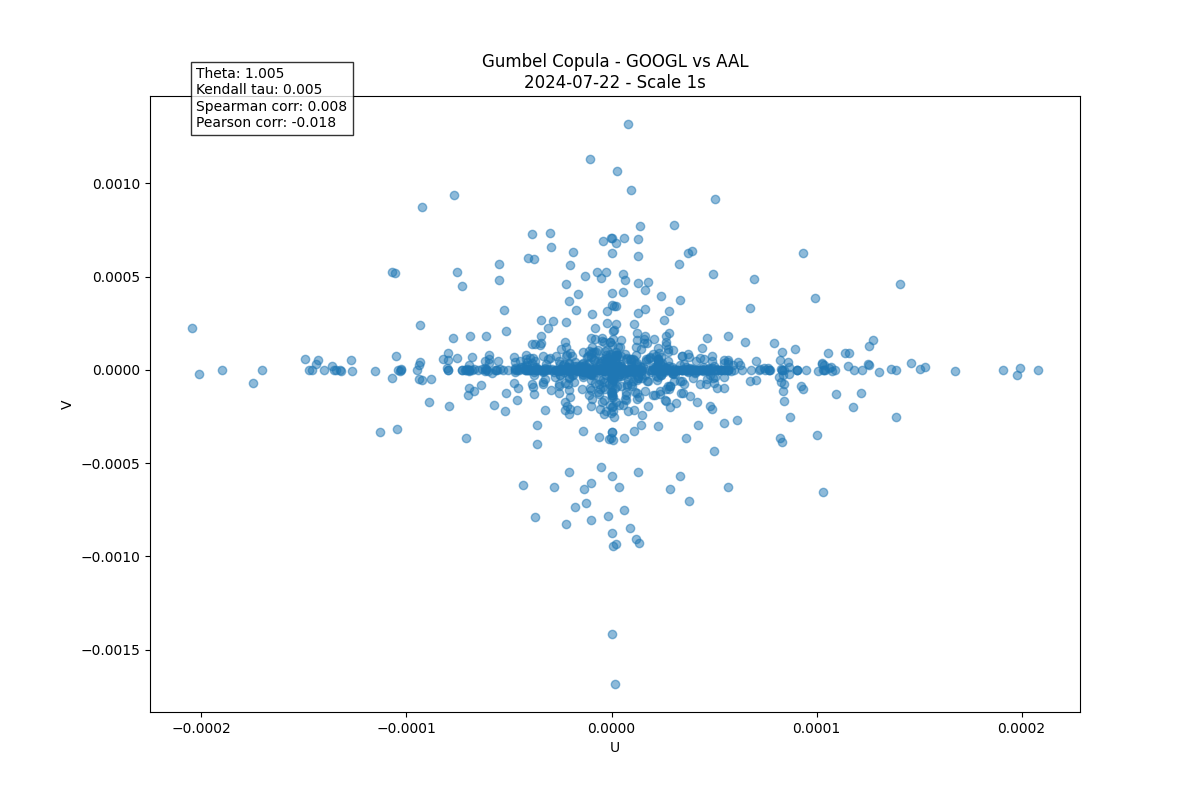
\includegraphics[width=0.8\textwidth]{GOOGL_AAL_2024-07-22_1s.png}
    \caption{Copule de Gumbel estimée pour la paire GOOGL-AAL le 22 juillet 2024 à l'échelle 1s. Les paramètres estimés montrent une faible dépendance ($\theta = 1.005$, $\tau = 0.005$), cohérente avec l'hypothèse d'indépendance conditionnelle à haute fréquence.}
    \label{fig:copula_example}
\end{figure}




\subsection{Synthèse des analyses de dépendance et stationnarité}

L'analyse conjointe des copules et de la stationnarité nous permet de tirer plusieurs conclusions importantes sur la nature des dépendances dans les marchés haute fréquence :

\begin{itemize}
    \item Les séries temporelles présentent une indépendance conditionnelle forte à l'échelle microscopique, confirmée par la faiblesse des dépendances capturées par les copules à ces échelles ($\tau < 0.2$ pour $\Delta t < 1\text{ms}$).
    
    \item Les changements de régime majeurs sont synchronisés entre les différents actifs, comme observé notamment lors de l'annonce des taux de la Fed le 18 septembre 2024, suggérant une source commune de non-stationnarité.
    
    \item La structure de dépendance évolue avec l'échelle temporelle : alors que les prix sont largement indépendants à l'échelle microscopique, des motifs de dépendance plus forts émergent aux échelles plus longues, particulièrement en période de stress.
\end{itemize}

Ces résultats soulignent l'importance d'une approche multi-échelle dans l'analyse des marchés haute fréquence, où les propriétés statistiques des séries de prix varient significativement selon l'horizon temporel considéré.

\begin{figure}[h!]
\centering
    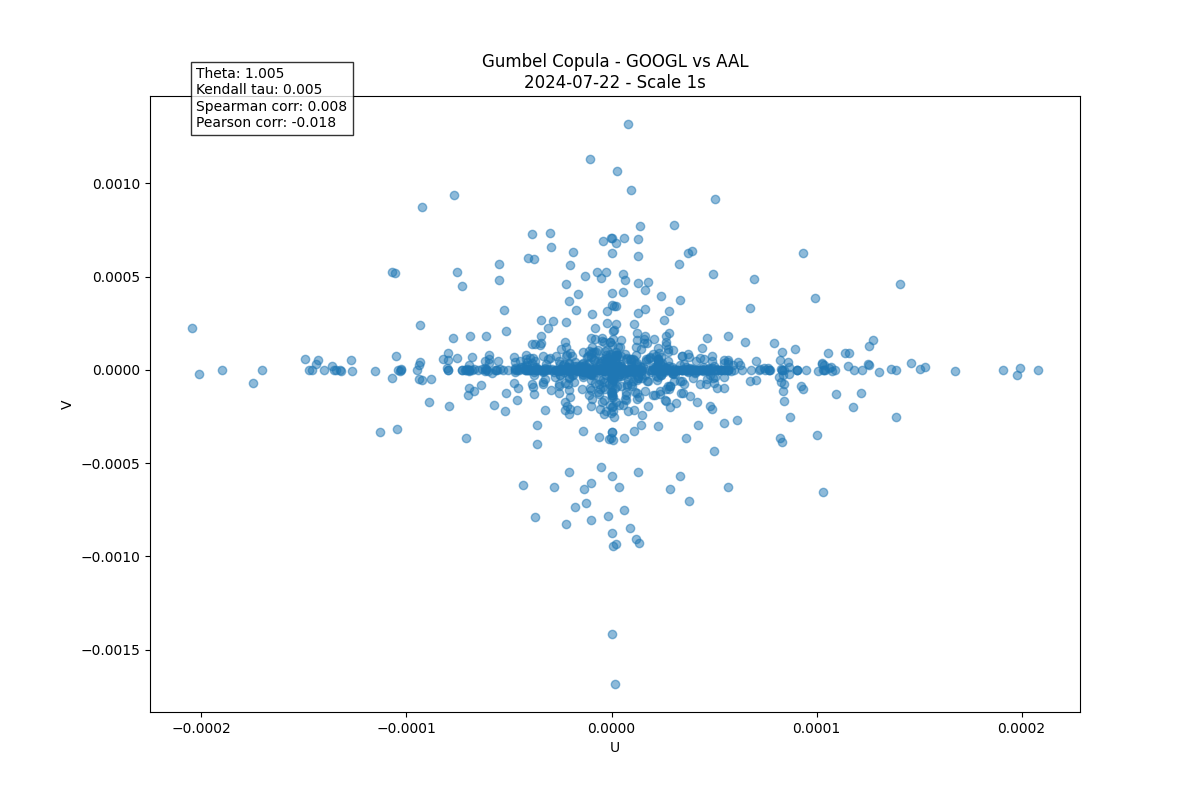
\includegraphics[width=0.8\textwidth]{GOOGL_AAL_2024-07-22_1s.png}
    \caption{Copule de Gumbel estimée pour la paire GOOGL-AAL le 22 juillet 2024 à l'échelle 1s. Les paramètres estimés montrent une faible dépendance ($\theta = 1.005$, $\tau = 0.005$), cohérente avec l'hypothèse d'indépendance conditionnelle à haute fréquence.}
    \label{fig:copula_example}
\end{figure}




\newpage
\section{Modélisation par processus de Hawkes}

\subsection{Présentation du modèle}

\subsection{Calibration et estimation}

\subsection{Application aux données de marché}

\newpage
\section{La théorie de Bouchaud sur la nature des sauts de prix}

La théorie de Bouchaud sur la nature des sauts de prix dans les marchés financiers repose sur une distinction fondamentale entre deux types d'événements extrêmes : les sauts exogènes (EMC - Efficient Market Class) et les sauts endogènes (SEC - Self-Exciting Class). Cette classification s'oppose à la théorie classique des marchés efficients qui stipule que tous les mouvements de prix significatifs sont nécessairement causés par des nouvelles externes.

\subsection{Caractéristiques des deux classes de sauts}

Les sauts exogènes (EMC) présentent les caractéristiques suivantes :
\begin{itemize}
    \item Ils surviennent de manière abrupte, sans signes précurseurs
    \item Ils sont suivis d'une relaxation rapide de la volatilité ($p_r^{EMC} \approx 0.7$)
    \item La volatilité post-saut descend souvent en dessous de son niveau initial
    \item Ils sont généralement associés à des annonces d'informations importantes
\end{itemize}

Les sauts endogènes (SEC) se distinguent par :
\begin{itemize}
    \item Une augmentation progressive de la volatilité avant le saut
    \item Une relaxation plus lente après le saut ($p_r^{SEC} \approx 0.4$)
    \item Un profil plus symétrique entre la phase de croissance et de décroissance
    \item L'absence de nouvelles externes significatives
\end{itemize}

\subsection{Le processus de Hawkes comme modèle explicatif}

Le modèle mathématique sous-jacent est un processus de Hawkes avec un noyau de mémoire en loi de puissance :

\begin{equation}
\lambda(t) = \lambda_0(t) + \sum_{t_i < t} \phi(t-t_i)
\end{equation}

où $\lambda(t)$ représente le taux instantané de mouvements de prix, $\lambda_0(t)$ est le taux exogène, et $\phi(\tau)$ est le noyau de mémoire qui capture la façon dont les événements passés influencent la probabilité d'événements futurs.

\subsection{Implications pour la compréhension des marchés}

Cette théorie a plusieurs implications importantes :

\begin{enumerate}
    \item Les marchés ne sont pas purement efficients : la majorité des sauts de prix significatifs (environ 97\%) sont endogènes
    \item Il existe des boucles de rétroaction entre les traders : le carnet d'ordres agit comme une source d'information publique qui peut amplifier de petites fluctuations
    \item La fragilité des marchés est intrinsèque : des mouvements de prix importants peuvent émerger sans nouvelle externe significative
    \item L'excès de volatilité observé empiriquement s'explique naturellement dans ce cadre
\end{enumerate}

Cette théorie s'inscrit dans une vision plus large des systèmes complexes, où des événements extrêmes peuvent émerger spontanément de l'interaction entre de nombreux agents, sans nécessiter de déclencheur externe majeur.

\newpage
\section*{Conclusion}

Ce mémoire apporte plusieurs contributions significatives à la compréhension des dynamiques de marché à haute fréquence et particulièrement à l'étude de l'impact des news sur les Limit Order Books. Notre approche, combinant analyse théorique et validation empirique, a permis de mettre en lumière plusieurs aspects fondamentaux de la microstructure des marchés.

\paragraph{\textbf{Caractérisation de la dynamique des prix}} Notre première contribution concerne la caractérisation fine de la dynamique des prix à différentes échelles temporelles. L'analyse de l'exposant de Hurst (H ≈ 0.7) révèle une persistance significative dans les mouvements de prix, suggérant l'existence de tendances locales exploitables. Cette observation est renforcée par l'étude des temps d'arrivée entre les changements de prix, qui suivent une distribution à queue lourde caractéristique des processus de Poisson inhomogènes.

\paragraph{\textbf{Identification des régimes de marché}} Notre seconde contribution porte sur la distinction entre les composantes endogènes et exogènes des variations de prix. Nous avons développé une méthodologie permettant d'identifier:
\begin{itemize}
    \item Les mouvements de prix résultant de la microstructure normale du marché (composante endogène)
    \item Les sauts de prix significatifs liés à l'arrivée d'informations externes (composante exogène)
    \item Les périodes de transition entre ces deux régimes
\end{itemize}

\paragraph{\textbf{Modélisation et prévision}} Notre troisième contribution est d'ordre méthodologique. En développant un cadre probabiliste rigoureux basé sur les processus de Hawkes, nous avons pu:
\begin{itemize}
    \item Modéliser la dynamique conjointe des ordres et des prix
    \item Quantifier l'impact des news sur la formation des prix
    \item Proposer des indicateurs d'alerte précoce pour les changements de régime
\end{itemize}

\paragraph{\textbf{Implications pratiques}} Ces résultats ont des implications importantes pour la pratique du trading algorithmique:
\begin{itemize}
    \item La calibration des stratégies de trading doit s'adapter au régime de marché identifié
    \item Les périodes post-news nécessitent des approches spécifiques de gestion du risque
    \item L'horizon temporel optimal des stratégies dépend de la persistance mesurée (H)
\end{itemize}

\paragraph{\textbf{Perspectives}} Plusieurs axes de recherche prometteurs émergent de ce travail:
\begin{itemize}
    \item L'extension du modèle à la prévision en temps réel des changements de régime
    \item L'intégration de sources d'information alternatives (réseaux sociaux, données alternatives)
    \item Le développement de stratégies de trading adaptatives basées sur la détection des régimes
\end{itemize}

Ces résultats ouvrent la voie à une nouvelle génération de modèles de trading algorithmique, capables de s'adapter dynamiquement aux conditions de marché et d'intégrer efficacement l'information exogène dans leurs décisions.

\newpage
\begin{thebibliography}{9}

\bibitem{chong2024minimax}
Carsten Chong, Marc Hoffmann, Yanghui Liu, Mathieu Rosenbaum, and Grégoire Szymanski.
\newblock Statistical inference for rough volatility: Minimax Theory.
\newblock \emph{arXiv preprint arXiv:2210.01214}, 2024.
\newblock URL: \url{https://arxiv.org/abs/2210.01214}.

\bibitem{chong2024clt}
Carsten H. Chong, Marc Hoffmann, Yanghui Liu, Mathieu Rosenbaum, and Grégoire Szymanski.
\newblock Statistical inference for rough volatility: Central limit theorems.
\newblock \emph{The Annals of Applied Probability}, 34(3), 2024.
\newblock DOI: \href{http://dx.doi.org/10.1214/23-AAP2002}{10.1214/23-aap2002}.

\end{thebibliography}

\end{document}